%%%%%%%%%%%%%%%%%%%%%%%%%%%%%%%%%%%%%%%%%%%%%%%%%%%%%%%%%%%%%%%%%%%%%%%%
%     LaTeX source code to approximate a NIST Technical report
%	  Instructions for authors: tinyurl.com/techpubsnist
%	DOI watermark will be added on final PDF
% 	Developed by K. Miller, kmm5@nist.gov
%	Last updated: 26-March-2019
%%%%%%%%%%%%%%%%%%%%%%%%%%%%%%%%%%%%%%%%%%%%%%%%%%%%%%%%%%%%%%%%%%%
\documentclass[12pt]{article}
\usepackage{adjustbox}
\usepackage{amsmath}
\usepackage{amsfonts}   % if you want the fonts
\usepackage{amssymb}    % if you want extra symbols
\usepackage{booktabs}
\usepackage{bm}
\usepackage{chemformula}
\usepackage{float}
%\usepackage{fourier}

\usepackage[hang,flushmargin,bottom]{footmisc} % footnote format
\usepackage{graphicx}   % need for figures
\usepackage{mathptmx}
\usepackage{multicol}
\usepackage{physics}
\usepackage{rotating}
\usepackage{secdot}
\usepackage{siunitx} % Formats the units and values
\usepackage{tabulary}
\usepackage{textgreek}
\usepackage{textcomp}
\usepackage{tikz}
\usepackage[newparttoc]{titlesec}
\usepackage[utf8]{inputenc}
\usepackage{xcolor}
\usepackage{footmisc}
\titleformat{\section}{\normalsize\bfseries}{\thesection.}{1em}{}	% required for heading numbering style
\titleformat*{\subsection}{\normalsize\bfseries}

\usepackage{tocloft}	% change typeset, titles, and format list of appendices/figures/tables
\renewcommand{\cftdot}{}	
\renewcommand{\contentsname}{Table of Contents}
\renewcommand{\cftpartleader}{\cftdotfill{\cftdotsep}} % for parts
\renewcommand{\cftsecleader}{\cftdotfill{\cftdotsep}}
\renewcommand\cftbeforesecskip{\setlength{4pt}{}}
\addtolength{\cftfignumwidth}{1em}
\renewcommand{\cftfigpresnum}{\figurename\ }
\addtolength{\cfttabnumwidth}{1em}
\renewcommand{\cfttabpresnum}{\tablename\ }
\setlength{\cfttabindent}{0in}    %% adjust as you like
\setlength{\cftfigindent}{0in}

\usepackage{enumitem}         % to control spacing between bullets/numbered lists

\usepackage[numbers,sort&compress]{natbib} % format bibliography
\renewcommand{\bibsection}{}
\setlength{\bibsep}{0.0pt}

\usepackage[hidelinks]{hyperref}
\hypersetup{
	colorlinks = true,
urlcolor ={blue},
citecolor = {.},
linkcolor = {.},
anchorcolor = {.},
filecolor = {.},
menucolor = {.},
runcolor = {.}
pdftitle={},%%put title here to auto-fill properties of the PDF
pdfsubject={},%%put abstract here
pdfauthor={}, %%put author list here
pdfkeywords={} %%put keywords here
}
\urlstyle{same}

\usepackage{epstopdf} % converting EPS figure files to PDF

\usepackage{fancyhdr, lastpage}	% formatting document, calculating number of pages, formatting headers
\setlength{\topmargin}{-0.5in}
\setlength{\headheight}{39pt}
\setlength{\oddsidemargin}{0.25in}
\setlength{\evensidemargin}{0.25in}
\setlength{\textwidth}{6.0in}
\setlength{\textheight}{8.5in}

\usepackage{caption} % required for Figure labels
\captionsetup{font=small,labelfont=bf,figurename=Fig.,labelsep=period,justification=raggedright}

%%%%%%%%%%% !!!!!! REQUIRED - FILL OUT METADATA HERE !!!!!!!! %%%%%%%%%%%%%%
%  	Report Number - fill in Report Number sent to you (see info below)
%   DOI Statement - fill in DOI sent to you
%   Month Year - fill in Month and Year of Publication
%%%%%%%%%%%%%%%%%%%%%%%%%%%%%%%%%%%%%%%%%%%%%%%%%%%%%%%%%%%%%%%%%%%%%%%%%%%%%%%%%%%%%%
\newcommand{\pubnumber}{XXXX}
\newcommand{\DOI}{https://doi.org/10.6028/NIST.TN.XXXX}
\newcommand{\monthyear}{August 2019}


\newcommand*\chem[1]{\ensuremath{\mathrm{#1}}}

\newcommand\numberthis{\addtocounter{equation}{1}\tag{\theequation}}

%%%%%%%%%%%%%%%%%%%%%%%%%%%%%%%%%%%%%%%%%%%%%%%%%%%%%%%%%%%%%%%%%%%%
%   	BEGIN DOCUMENT
%%%%%%%%%%%%%%%%%%%%%%%%%%%%%%%%%%%%%%%%%%%%%%%%%%%%%%%%%%%%%%%%%%%%
\begin{document}
	\urlstyle{rm} % Format style of \url
	
%%%%%%%%%%%%%%%%%%%%%%%%%%%%%%%%%%%%%%%%%%%%%%%%%%%%%%%%%%%%%%%%%%%%
%   Cover Page is REQUIRED and must contain the information
%	displayed here, at a minimum. Additional artwork may be included
%	(e.g., official project/conference logo, etc.).
%	Pub Number automated based on metadata
%%%%%%%%%%%%%%%%%%%%%%%%%%%%%%%%%%%%%%%%%%%%%%%%%%%%%%%%%%%%%%%%%%%%
	\begin{titlepage}
		\begin{flushright}
%%%%%%%%%%%%%%%%%%%%%%%%%%%%%%%%%%%%%%%%%%%%%%%%%%%%%%%%%%%%%%%%%%%%
% 	Automated based on metadata - delete if not applicable
%%%%%%%%%%%%%%%%%%%%%%%%%%%%%%%%%%%%%%%%%%%%%%%%%%%%%%%%%%%%%%%%%%%%
\LARGE{\textbf{NIST Technical Note \pubnumber}}\\
\vfill
%%%%%%%%%%%%%%%%%%%%%%%%%%%%%%%%%%%%%%%%%%%%%%%%%%%%%%%%%%%%%%%%%%%%
%	Title
%%%%%%%%%%%%%%%%%%%%%%%%%%%%%%%%%%%%%%%%%%%%%%%%%%%%%%%%%%%%%%%%%%%%
\Huge{\textbf{The Structure of Medium-Scale Pool Fires}}\\
\vfill
%%%%%%%%%%%%%%%%%%%%%%%%%%%%%%%%%%%%%%%%%%%%%%%%%%%%%%%%%%%%%%%%%%%%
%	Authors - add complete list of authors, affiliations will be
%   added on title page
%%%%%%%%%%%%%%%%%%%%%%%%%%%%%%%%%%%%%%%%%%%%%%%%%%%%%%%%%%%%%%%%%%%%
\large Ryan Falkesntein-Smith\\
\large Anthony Hamins\\
\large Kunhyuk Sung\\
\large Jian Chen\\
\vfill
%%%%%%%%%%%%%%%%%%%%%%%%%%%%%%%%%%%%%%%%%%%%%%%%%%%%%%%%%%%%%%%%%%%%
%	The DOI is automated based on metadata.	
%%%%%%%%%%%%%%%%%%%%%%%%%%%%%%%%%%%%%%%%%%%%%%%%%%%%%%%%%%%%%%%%%%%%
\normalsize This publication is available free of charge from:\\
\DOI\\
\vfill
%%%%%%%%%%%%%%%%%%%%%%%%%%%%%%%%%%%%%%%%%%%%%%%%%%%%%%%%%%%%%%%%%%%%
%	NIST LOGO - keep as-is
%%%%%%%%%%%%%%%%%%%%%%%%%%%%%%%%%%%%%%%%%%%%%%%%%%%%%%%%%%%%%%%%%%%%


\includegraphics[width=0.3\linewidth]{NIST-logo}\\


\end{flushright}
\end{titlepage}
\begin{titlepage}
%%%%%%%%%%%%%%%%%%%%%%%%%%%%%%%%%%%%%%%%%%%%%%%%%%%%%%%%%%%%%%%%%%%%
%	Title Page is REQUIRED
%%%%%%%%%%%%%%%%%%%%%%%%%%%%%%%%%%%%%%%%%%%%%%%%%%%%%%%%%%%%%%%%%%%%
\begin{flushright}
%%%%%%%%%%%%%%%%%%%%%%%%%%%%%%%%%%%%%%%%%%%%%%%%%%%%%%%%%%%%%%%%%%%%
%   Publication Series & Number - automated
%%%%%%%%%%%%%%%%%%%%%%%%%%%%%%%%%%%%%%%%%%%%%%%%%%%%%%%%%%%%%%%%%%%%
\LARGE{\textbf{NIST Technical Note \pubnumber}}\\
\vfill
%%%%%%%%%%%%%%%%%%%%%%%%%%%%%%%%%%%%%%%%%%%%%%%%%%%%%%%%%%%%%%%%%%%%
%	Title
%%%%%%%%%%%%%%%%%%%%%%%%%%%%%%%%%%%%%%%%%%%%%%%%%%%%%%%%%%%%%%%%%%%%
\Huge{\textbf{The Structure of Medium-Scale Pool Fires}}\\
\vfill
%%%%%%%%%%%%%%%%%%%%%%%%%%%%%%%%%%%%%%%%%%%%%%%%%%%%%%%%%%%%%%%%%%%%
%	Author Order and Grouping. Always identify the primary author/creator first (s/he does not have to be a NIST author). For publications with multiple authors, group authors by their organizational affiliation. The organizational groupings and the names within each grouping should generally be ordered by decreasing level of contribution.
%	For non-NIST authors, list their city and state below their organization name.
%	For NIST authors, include the Division and Laboratory names (but do not include their city and state).
%%%%%%%%%%%%%%%%%%%%%%%%%%%%%%%%%%%%%%%%%%%%%%%%%%%%%%%%%%%%%%%%%%%%
\normalsize Ryan Falkenstein-Smith\\
Anthony Hamins\\
Kunhyuk Sung\\
Jian Chen\\
\large
\textit{Fire Research Division}\\
\textit{Engineering Laboratory}\\
\vspace{12pt}
\vfill
%%%%%%%%%%%%%%%%%%%%%%%%%%%%%%%%%%%%%%%%%%%%%%%%%%%%%%%%%%%%%%%%%%%%
%   DOI Statement - automated
%%%%%%%%%%%%%%%%%%%%%%%%%%%%%%%%%%%%%%%%%%%%%%%%%%%%%%%%%%%%%%%%%%%%
\normalsize This publication is available free of charge from:\\
\DOI\\
\vfill
%%%%%%%%%%%%%%%%%%%%%%%%%%%%%%%%%%%%%%%%%%%%%%%%%%%%%%%%%%%%%%%%%%%%
%   Date - Month and Year - automated
%%%%%%%%%%%%%%%%%%%%%%%%%%%%%%%%%%%%%%%%%%%%%%%%%%%%%%%%%%%%%%%%%%%%
\normalsize \monthyear
\vfill
%%%%%%%%%%%%%%%%%%%%%%%%%%%%%%%%%%%%%%%%%%%%%%%%%%%%%%%%%%%%%%%%%%%%
%  Department of Commerce LOGO - leave as-is
%%%%%%%%%%%%%%%%%%%%%%%%%%%%%%%%%%%%%%%%%%%%%%%%%%%%%%%%%%%%%%%%%%%%	


\includegraphics[width=0.18\linewidth]{DoC-logo}\\
\vfill
%%%%%%%%%%%%%%%%%%%%%%%%%%%%%%%%%%%%%%%%%%%%%%%%%%%%%%%%%%%%%%%%%%%%
%  Department of Commerce & NIST Leadership
%	will be updated as changes occur
%%%%%%%%%%%%%%%%%%%%%%%%%%%%%%%%%%%%%%%%%%%%%%%%%%%%%%%%%%%%%%%%%%%%
\footnotesize U.S. Department of Commerce\\
\textit{Wilbur L. Ross, Jr., Secretary}\\
\vspace{10pt}
National Institute of Standards and Technology\\
\textit{Walter Copan, NIST Director and Undersecretary of Commerce for Standards and Technology}
\end{flushright}
\end{titlepage}

\begin{titlepage}
%%%%%%%%%%%%%%%%%%%%%%%%%%%%%%%%%%%%%%%%%%%%%%%%%%%%%%%%%%%%%%%%%%%%
%   Disclaimer/CODEN page - required
%%%%%%%%%%%%%%%%%%%%%%%%%%%%%%%%%%%%%%%%%%%%%%%%%%%%%%%%%%%%%%%%%%%%
\begin{flushright}
\footnotesize  Certain commercial entities, equipment, or materials may be identified in this document in order to describe an experimental procedure or concept adequately. Such identification is not intended to imply recommendation or endorsement by the National Institute of Standards and Technology, nor is it intended to imply that the entities, materials, or equipment are necessarily the best available for the purpose.\\
\vfill
%%%%%%%%%%%%%%%%%%%%%%%%%%%%%%%%%%%%%%%%%%%%%%%%%%%%%%%%%%%%%%%%%%%%
%   This secton automated - do not change
%%%%%%%%%%%%%%%%%%%%%%%%%%%%%%%%%%%%%%%%%%%%%%%%%%%%%%%%%%%%%%%%%%%%
\normalsize \textbf{National Institute of Standards and Technology Technical Note \pubnumber\\
Natl. Inst. Stand. Technol. Tech. Note \pubnumber, \pageref{LastPage} pages (\monthyear)} \\
\textbf{CODEN: NTNOEF}\\
\vspace{12pt}
\textbf{This publication is available free of charge from: \DOI}
\vfill
\end{flushright}
\end{titlepage}
%%%%%%%%%%%%%%%%%%%%%%%%%%%%%%%%%%%%%%%%%%%%%%%%%%%%%%%%%%%%%%%%%%%%
%   Start front matter - page number starts with "i"
%%%%%%%%%%%%%%%%%%%%%%%%%%%%%%%%%%%%%%%%%%%%%%%%%%%%%%%%%%%%%%%%%%%%
\section*{Abstract}
This report documents a series of time-averaged gas species measurements made along the centerline of methanol, ethanol, and acetone pool fires steadily burning in a quiescent environment. All gas species measurements are obtained using a Gas Chromatograph/ Mass Spectrometer system (GC/MSD). The volume fraction of each species was calculated via the number of moles identified by the GC/MSD at each location ({\bf Kevin -- this statement doesn't explain very much}). Soot mass fractions are simultaneously measured during the gas sampling process. The gas species volume and soot mass fractions are compared at different heights within the fire and across a variety of different fuels. Other fire parameters are measured as well, including time-averaged temperature measurements and mass burning rates.
\section*{Keywords}
\normalsize Acetone, Ethanol, Gas species measurements, Methanol, Liquid pool fires \\
\pagebreak
%%%%%%%%%%%%%%%%%%%%%%%%%%%%%%%%%%%%%%%%%%%%%%%%%%%%%%%%%%%%%%%%%%%%
%   Table of Contents is required
% 	List of Tables & Figures required if more than 5 tables/figures
%%%%%%%%%%%%%%%%%%%%%%%%%%%%%%%%%%%%%%%%%%%%%%%%%%%%%%%%%%%%%%%%%%%%
\begin{center}
	\tableofcontents
	\listoftables
	\listoffigures
\end{center}
\pagebreak
%%%%%%%%%%%%%%%%%%%%%%%%%%%%%%%%%%%%%%%%%%%%%%%%%%%%%%%%%%%%%%%%%%%%
%   Start body of text - page number starts with "1"
%%%%%%%%%%%%%%%%%%%%%%%%%%%%%%%%%%%%%%%%%%%%%%%%%%%%%%%%%%%%%%%%%%%%
\section{Introduction}
\label{sec:intro}
Computational fluid dynamics (CFD) models are an important component of performance-based design in fire protection engineering. A requirement of their acceptance in the design process is that these models be verified and validated, the latter of which involves comparison with experimental measurements. The primary objective of this report is to provide data for use in fire model validation.

A pool fire is a fundamental focus of study in fire science. The fuel surface is isothermal, flat and horizontal, providing a well-defined boundary condition for modeling. Fuel and product species concentrations and temperatures have a significant influence on the heat feedback to the fuel surface, which directly affects the burning rate. A zone of particular interest is the fuel rich-core between the flame and the pool surface, where gas species can absorb energy that would otherwise have been transferred to the fuel surface. Few studies in the literature have reported local chemical species measurements within the flame envelop.

The purpose of this study is to characterize the spatial distribution of the principal chemical species in moderate-scale liquid pool fires steadily burning in a well-ventilated, quiescent environment. Here, methanol, ethanol, and acetone are the fuels of interest. Contrary to ethanol and acetone, fires established using methanol are unusual as no carbonaceous soot is present or emitted. These particular fuels are selected for research since the measurements complement results from previous studies, including analyses of the mass burning rate, the temperature and velocity fields, radiative emission, flame height, and pulsation frequency~\cite{Fisher1987,Hamins2016}.


\clearpage

\section{Description of Experiments}
\label{sec:Experiments}

Descriptions of previous pool fire experiments are found in Refs.~\cite{Hamins2016,Hamins1994,Hamins1991,Hamins1996,Lock2008}.

\subsection{Pool Burner Setup}
\label{ssec:Pool_Burner_Setup}

The experiments are conducted under a canopy hood surrounded by a cubical enclosure 2.5~m on a side made of a double layer of wire-mesh screen (5 mesh/cm) to reduce the impact of room ventilation. All measurements are made once the mass burning rate reaches a steady-state, achieved approximately 10~min after ignition.

The circular, stainless-steel burn pan has an outer diameter of 30~cm, a depth of 15~cm, and a wall thickness of 1.6~mm. The lip of the burner is positioned 30~cm above the floor. As shown in Fig.~\ref{fig:Pool Burner}, the burner is placed within an overflow basin, which extends 3~cm beyond the burner wall.  The bottom of the burner is maintained at a constant temperature by flowing water ($20 \; ^\circ \hbox{C} \pm 3 \; ^\circ \hbox{C}$)  through the basin. A fuel level indicator is positioned near the center of the burner to maintain a consistent surface level.

\begin{figure}[h!]
	\centering
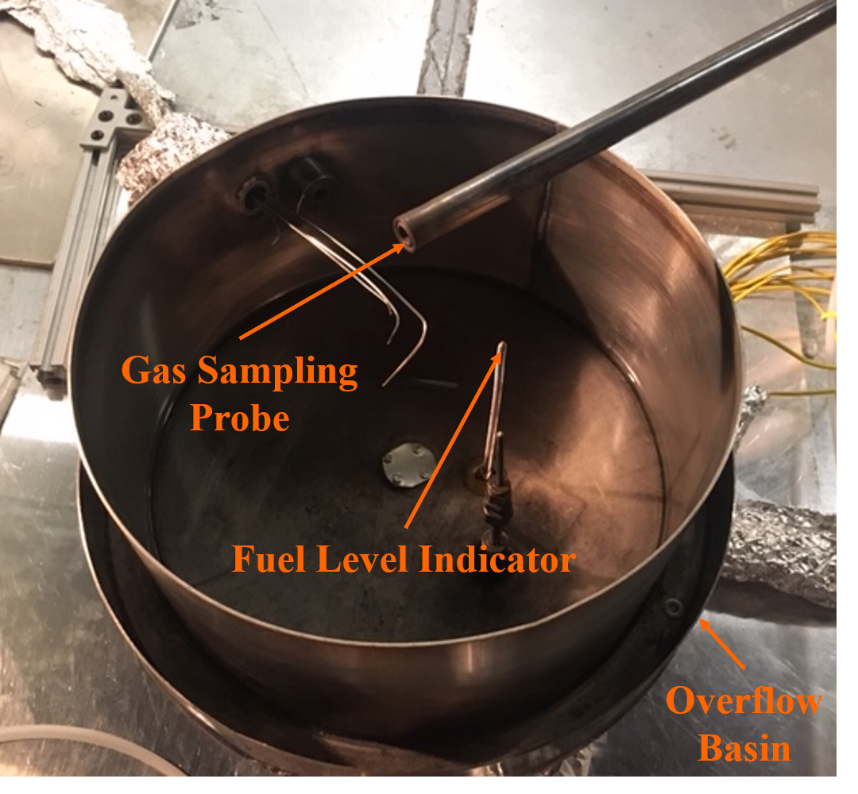
\includegraphics[width=10.0cm,keepaspectratio]{Pool_Burner.png}
	\caption[Photograph of the burner]{The 30~cm burner with fuel level indicator, overflow section, and quenching probe}
	\label{fig:Pool Burner}
\end{figure}

Fuel to the burner is gravity fed from a reservoir positioned on a mass load cell located outside the enclosure and monitored by a data acquisition system (DAQ). As shown in Fig.~\ref{fig:Fuel_Level}, the fuel level is monitored via a fuel flow operator. The operator is able to observe a close up of a slightly discernible dimple (approximately \SI{2}{mm}) made from the fuel level indicator on the fuel surface using a live video feed. The fuel level is controlled by manually adjusting the fuel flow using a needle valve. The fuel surface is maintained \SI{10}{mm} below the burner rim to match previous experimental conditions \cite{Fisher1987,Hamins2016,Kim2019,Weckman1996}

\begin{figure}[h!]
	\centering
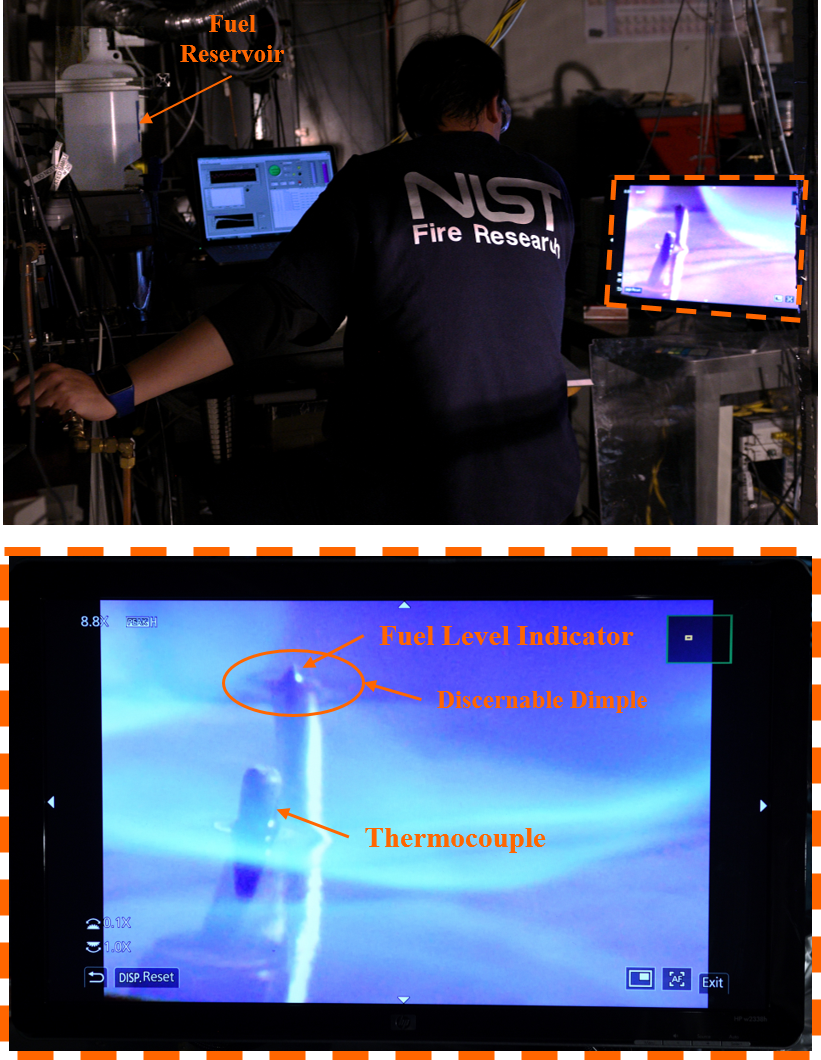
\includegraphics[width=14.0cm,keepaspectratio]{Monitoring_Fuel_Level_A.png}
	\caption[Photo of fuel flow operator monitoring the fuel level via live video feed (top) and a magnified image of the live video feed used to maintain a consistent fuel level relative to the fuel level indicator (bottom)]{Photo of fuel flow operator monitoring the fuel level via live video feed (top) and a magnified image of the live video feed used to maintain a consistent fuel level relative to the fuel level indicator (bottom)}
	\label{fig:Fuel_Level}
\end{figure}



The heat release rate, $\dot{Q}$, is the product of the time-averaged mass burning rate, $\dot{m}$, and the heat of combustion, $\Delta H_{c}$:
\begin{equation}\label{eq:Heat_release_rate}
\dot{Q}= \dot{m}~\Delta H_{c}
\end{equation}
The heat of the combustion is provided by Ref.~\cite{Dippr} and reported in Table~\ref{tab:Pool_Fire_Parameters_Table}. The uncertainty of the mass burning rate is discussed in Appendix~\ref{ssec:Mass_Burning_Flux}. The uncertainty of the heat release rate is discussed in Appendix~\ref{ssec:Heat_Release_Rate}.

The mean flame height, $L_{\rm{f}}$, is estimated from 3600~frames of high-resolution video of the experiments using MATLAB’s Image Processing Toolbox\footnote{\label{fn:product} Certain commercial products are identified in this report to specify adequately the equipment used. Such identification does not imply a recommendation by the National Institute of Standards and Technology, nor does it imply that this equipment is the best available for the purpose.}. Imported color images are decomposed into binary (i.e., black and white) images using a pre-set threshold level. The flame height for a single frame is defined as the distance between the pool surface and flame tip. All measurements are repeated, then averaged to provide the mean flame height. A description of the uncertainty analysis for the mean flame height is described in Appendix~\ref{ssec:Mean_Flame_Height}.

\subsection{Centerline Temperature Measurements}
\label{ssec:Temperature_Measurements}

Time-averaged temperature measurements are made along the vertical centerline of the fire plumes. An S-type (Pt 10\% Rh/Pt), bare-wire, fine diameter thermocouple with a diameter of \SI{50}{\micro\metre} (OMEGA P10R-001\footref{fn:product}) is positioned using a computer-controlled traverse. Temperature measurements are sampled at \SI{250}{Hz} for \SI{2}{min}, or approximately 300~pulsing cycles \cite{Wang2019}.

The thermal inertia and radiative heat loss associated with the thermocouple are corrected following Shaddix's method~\cite{Shaddix1999}. The energy balance on the thermocouple bead considered the convective, radiative, and conductive heat transfer and can be expressed as:
\begin{equation}\label{eq:Thermocouple_Bead_Energy_Balance}
{\dot{Q}_{\rm con}+\dot{Q}_{\rm rad}}= \rho_{\rm b}~c_{\rm b}~V_{\rm b}\frac{{\rm d}T_{\rm b}}{{\rm d}t}
\end{equation}
where $\dot{Q}_{\rm con}$ and $\dot{Q}_{\rm rad}$ are the net rate of convective and radiative heat transfer, respectively, and $\rho_{\rm b}$, $c_{\rm b}$, $V_{\rm b}$ are the density, specific heat and volume of the bead, respectively. The thermal inertia effect is related to the thermocouple time constant, $\tau$, and can be incorporated into Eq.~(\ref{eq:Thermocouple_Bead_Energy_Balance}) to correct the temperature measurement. The energy balance from Eq.~(\ref{eq:Thermocouple_Bead_Energy_Balance}) can be simplified to solve for the corrected gas temperature.
\begin{equation}\label{eq:Thermocouple_Bead_Correction}
{T_{\rm g}(t)}= T_{\rm b}(t) + \tau \, \frac{{\rm d}T_{\rm b}}{{\rm d}t} + \frac{\epsilon\sigma}{h}\left({T_{\rm b}(t)}^4-{T_{\rm surr}(t)}^4\right)
\end{equation}
where $T_{\rm g}$ is the effective temperature of the gas, $T_{\rm b}$ is the measured bead temperature, $T_{\rm surr}$ is the effective temperature of the surroundings, $\sigma=5.67 \times 10^{-11} \; {\rm kW}/({\rm m}^2{\rm K}^4)$ is the Stefan-Boltzmann constant, $\epsilon$ is the thermocouple emissivity, and $h$ is the convective heat transfer coefficient of the gas flow near the bead. Specific heat of thermocouple bead is taken from Ref.~\cite{Jaeger1939}. The temperature dependent emissivity of the platinum was taken from Ref.~\cite{Incropera2007}. The coefficients of $h$ and $\tau$ and are further defined as:
\begin{equation}\label{eq:h_eqn}
h=\frac{{\rm Nu} \, k_{\rm g}}{D_{\rm b}}  \quad ; \quad \tau= \frac{\rho_{\rm b} \, c_{\rm b} \, {D_{\rm b}}^2}{6 \, {\rm Nu} \, k_{\rm g}}
\end{equation}
where $k_{\rm g}$ is the thermal conductivity of the gas and $D_{\rm b}$ is the diameter of the bead. The Nusselt number, Nu, for the bead was calculated using the Ranz-Marshall correlation~\cite{Shaddix1999}, as shown in the Eq.~(\ref{eq:Nu_number}).
\begin{equation}\label{eq:Nu_number}
{\rm Nu} = 2+{\textrm{Re}_{\rm D}}^{\frac{1}{2}}+\textrm{Pr}^{\frac{1}{3}}
\end{equation}
The temperature-dependent gas properties for, Reynolds number, Re, and Prandtl number, Pr, are taken as those of air from Ref.~\cite{Dippr}. The gas velocity was assumed to be equal to 2 m/s to determine the Re. Calculations showed that the corrected temperature had little sensitivity on the magnitude of the velocity between values of \SI{1}{ m/s} and \SI{3}{m/s}, which is consistent with the results of Shaddix~\cite{Shaddix1999}. The uncertainty of the time-averaged temperature measurements are discussed in Appendix~\ref{sec:Uncertainty_Temperature_Measurements}.

\subsection{Measuring the Volume Fraction of Gas Species via GC/MSD}
\label{ssec:Gas_Species_Setup}

Gas-species measurements are made using an Agilent 5977E Series GC/MSD fitted with a thermal conductivity detector (TCD). The GC/MSD is able to quantify a variety of stable reactants, intermediates, and combustion product species collected from the pool fire. The GC/MSD is equipped with a \SI{2}{ml} sample loop maintained at \SI{200}{\degree C}. Chromatographic separation of species is achieved using a Select for Permanent Gases-Dual Column (CP7430) comprised of mole-sieve and Porapak Q columns working in parallel and using a helium carrier gas. The sample analysis time is \SI{62}{min} wherein the carrier gas flow leading into the TCD and MSD is \SI{3}{ml/min} and \SI{1}{ml/min}, respectively. During the analysis, the GC oven temperature is maintained at \SI{30}{\degree C} for \SI{12}{min}, then ramped at \SI{8}{\degree C/min} for \SI{2}{min} until a temperature of \SI{300}{\degree C} is reached.

Figure~\ref{fig:Experimental_Setup} displays the flow diagram for gas sampling into the GC/MSD. The gases are extracted by a vacuum pump located downstream of the GC/MSD. Gas samples are collected using a quenching probe. The quenching probe is composed of two concentric, stainless-steel tubes with outer annular coolant flow and inner, extracted, gas-sample flow. The inner and outer tube diameters are \SI{8}{mm}and \SI{16}{mm}, respectively. Water at \SI{90}{\degree C} flows through the sampling probe for the duration of the experiment. The remainder of the sampling line leading into the GC/MSD is heated with electrical, heating tape to \SI{140}{\degree C} to prevent condensation of water and liquid fuels through the line.

\begin{sidewaysfigure}[!]
	\centering
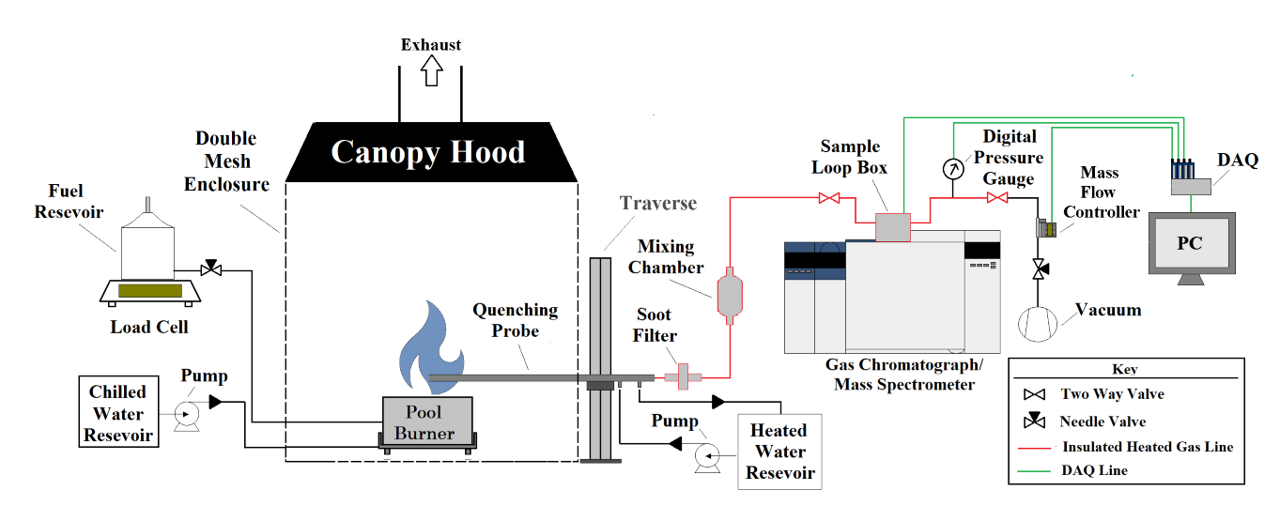
\includegraphics[width=\textwidth,keepaspectratio]{Experimental_Setup.png}
	\caption[A schematic of the gas sampling procedure]{A schematic of the extraction sampling setup used to transport gas samples from the pool fire to the GC/MSD.}
	\label{fig:Experimental_Setup}
\end{sidewaysfigure}

Gas sampling is conducted for a minimum of \SI{12}{min}, ensuring that the gas sample is completely swept through the GC/MSD sample loop. The gas sampling period varies from \SI{12}{min} to \SI{25}{min} depending on the sampling location within the fire. The sampling flow is controlled using a mass flow controller (Alicat Scientific MC-Series\footref{fn:product}) located in front of the vacuum pump within the sampling line. During the gas sampling procedure, the volumetric flow is approximately \SI{200}{ml/min} and recorded, using a DAQ, at \SI{2}{\hertz} for the entire duration of the gas sampling procedure. The mass flow controlled also provides temperature readings of its internal gas flow.

After the gas sampling period, two quarter-turn valves located on opposite ends of the GC/MSD sample loop within the sampling line are closed. Once the sampled gas reaches equilibrium, pressure measurements, obtained from a digital pressure gauge (OMEGA DPG409-030DWU), and temperature measurements, acquired by a K-type thermocouple located at the GC/MSD sample loop injection port, are collected at \SI{2}{\hertz} for \SI{50}{s}. After collecting pressure and temperature measurements, the sampled gas is injected into the GC/MSD.

The mean volume fraction of a given species, $\bar{X}_{i}$, is the ratio of the number of moles of a given gas species, $n_{i}$, and the total number of moles identified by the GC/MSD, $n_{\rm tot}$. The total number of moles is determined from the summation of moles for each species identified by either the TCD or MSD.
\begin{equation}\label{eq:volume_fraction}
  	\bar{X}_{i}= \frac{n_{i}}{n_{\rm tot}}
\end{equation}
The mean mass fraction, $\bar{Y}_{i}$, of a given species $i$ is calculated from the measured volume fraction, $\bar{X}_{i}$, using the following expression:
\begin{equation}\label{eq:mass_fraction}
	\bar{Y}_{i}=\frac{\bar{X}_{i} \, {\textrm{W}_{i}}}{\sum{\bar{X}_{i} \, {\textrm{W}_{i}}}}
\end{equation}
where ${{\textrm{W}_{i}}}$ is the molecular weight of a given species.

All measurements using the GC/MSD are repeated at least twice at each location along the centerline of the pool fire. Gas species concentration measurements made at the same location are averaged. The variance in the volume fraction is a function of position and species. A detailed description of the uncertainty analysis for the gas species measurement and its calibration is discussed in Appendices~\ref{sec:UncertaintyGasSpecies} and \ref{sec:Uncertainty Analysis of Gas Species Calibrations}.

\subsection{Determining Soot Mass Fraction}
\label{ssec:Soot_Setup}

Soot mass fraction, $Y_{\rm s}$, is measured using a well established gravimetric technique~\cite{Choi1995}. Soot is filtered out of the gas stream using a stainless steel particulate filter holder (PALL 2220).  Before an experiment, a desiccated \SI{47}{mm} polytetrafluoroethylene (PTFE) filter is weighed and placed into its holder. The filter holder is positioned within the gas sampling line behind the quenching probe and heated with tape to approximately \SI{140}{\degree C} to prevent condensation of water and liquid fuels on the filter. After sampling, the filter is removed and dried in a desiccator. After drying for 48~h, the filter’s final weight is measured. Approximately \SI{1}{mg} of soot is collected during the sampling period, which varies from 12~min to 25~min depending on the sampling location. The mass of the PTFE filter and cleaning patches were measured three times before and after each test\footnote{After some experiments, soot deposits were observed on the inner walls of the quenching probe. As shown in Fig.~\ref{fig:Soot_Probe_Setup}, dedicated gun cleaning patches were used to clean the inside of the quenching probe. Patches are weighed immediately before and 48~h after cleaning the inside of the probe.}.

\begin{figure}[ht!]
	\centering
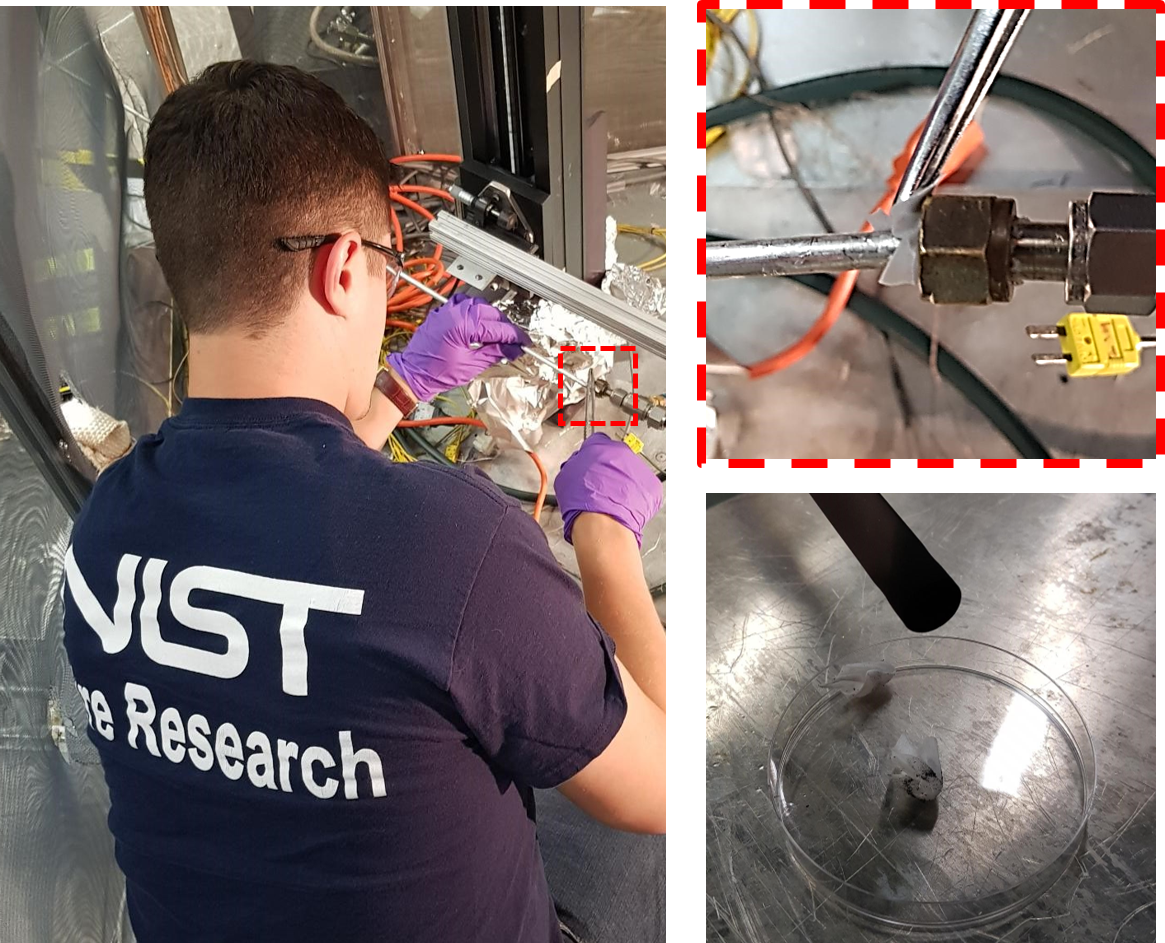
\includegraphics[width=15.0cm,keepaspectratio]{Soot_Probe.png}
	\caption[Process for cleaning soot probe]{Process of collecting soot from the internal walls of the quenching probe using gun cleaning patches}
	\label{fig:Soot_Probe_Setup}
\end{figure}

The soot mass fraction, $Y_{\rm s}$, is computed from the mass of the soot collected from the PTFE filter and gun cleaning patches, $m_{\rm s}$, the ratio of the mass flow controller's temperature reading, $T_{\infty}$, to the effective temperature of the gas calculated from Eq.~(\ref{eq:Thermocouple_Bead_Correction}), $T_{\rm g}$, the total mass of gas sampled, $m_{\rm tot}$, based on the mass flow controller readings:
\begin{equation}\label{eq:soot_mass_frac}
Y_{s}= \frac{m_{\rm s}}{m_{\rm tot}}\frac{T_{\infty}}{T_{\rm g}}
\end{equation}
The total mass of gas sampled is the product of the average volumetric flow rate measured by the mass flow controller, $\dot{V}$, the density of the sample gas injected into the GC/MSD, $\rho_{\rm g}$, and the gas sampling time, $\Delta t$.
\begin{equation}\label{eq:total_mass}
m_{t}= \dot{V} \, \rho_{g}\, \Delta t
\end{equation}
In Eq.~(\ref{eq:total_mass}), the density of the sample gas is determined from the total mass detected from the TCD and MSD, $m_{\rm tot}$, for the injected sample volume, $V_{\rm s}$.
\begin{equation}\label{eq:gas_density}
\rho_{\rm g}= \frac{m_{\rm tot}}{V_{\rm s}}
\end{equation}
A description of the soot mass fraction uncertainty is provided in Appendix~\ref{sec:Uncertainty_Soot_Frac}.




\clearpage

\section{Results}
\label{sec:Results}

This section presents the gas species and soot measurements made at incremental heights along the centerline of medium-scale pool fires using various fuels such as methanol, ethanol, and acetone.

\subsection{Flame Observations}
\label{ssec:Flame_Observations}

Figure~\ref{fig:Flame_Structure} displays a series of snapshots depicting a single pulsation cycle of the methanol, ethanol, and acetone fires. The pulsation frequency is approximately 3~Hz.
\begin{figure}[p]
	\centering
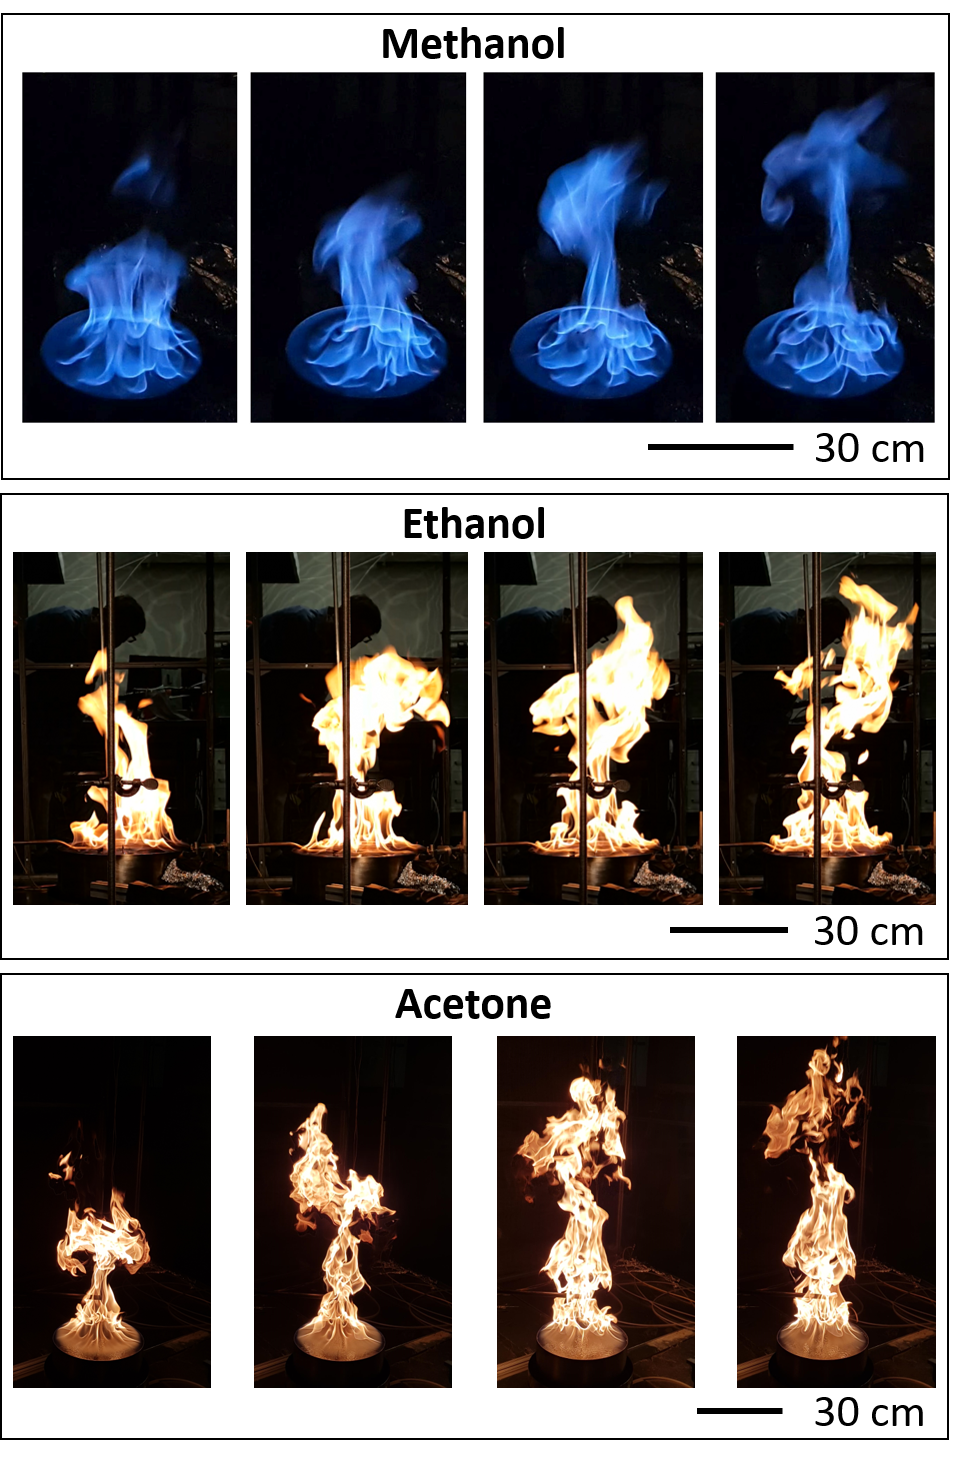
\includegraphics[width=5.0in,keepaspectratio]{Flame_Structure.png}
	\caption[Pool Fire Structures]{Flame structures of methanol (top), ethanol (middle), and acetone (bottom) pool fires during their pulsing cycles}
	\label{fig:Flame_Structure}
\end{figure}
The methanol fire has a pale blue color, whereas the ethanol and acetone fires are more luminous and yellow. The measured time-averaged burning rates and calculated heat release rates are listed in Table~\ref{tab:Pool_Fire_Parameters_Table}. The heat release rates are calculated from Eq.~(\ref{eq:Heat_release_rate}). The methanol fire has the lowest average flame height, followed by the ethanol, and then the acetone. The measured mean flame heights match Heskestad’s correlation~\cite{Heskestad1983} to within measurement uncertainty. The flame heights are also within the uncertainty bounds of measurements made by Kim~et~al.~\cite{Kim2019}.

\begin{table}[!ht]
\caption{List of measurements and thermochemical properties of fuels burning in a well-ventilated round 30~cm diameter pool fire burning in a quiescent environment. The uncertainties of measurements are discussed in detail in Appendix~\ref{sec:Uncertainty_Pool_Fire_Parameters}.}
\label{tab:Pool_Fire_Parameters_Table}
\centering
	\footnotesize
	\begin{tabular}{lccc}
\hline
%\\[0.0005cm]
\textbf{Parameter (units)} &\textbf{Methanol}& \textbf{Ethanol}& \textbf{Acetone}\\
\hline
\\[0.01cm]
Mass Burning Flux~(\si{g/{m^2 s}})		        &	12.4~$\pm$~1.1		&	13.9~$\pm$~0.8	&	17.6~$\pm$~2.7\\
\\[0.01cm]
Heat Release Rate~(\si{kW})		            	&	17.4~$\pm$~1.4		&	26.3~$\pm$~1.5	&	35.5~$\pm$~5.4\\
\\[0.01cm]
Mean Flame Height~(\si{cm})			            &	36.4~$\pm$~16.0		&	61.1~$\pm$~28.2	&	91.5~$\pm$~34.6\\
\\[0.01cm]
Heat of Combustion (kJ/g)~\cite{SFPE}			&	19.94				&	26.81			&	28.56			\\	
\\[0.01cm]
Carbon/Hydrogen Ratio				         	&	1/4			&	1/3		&	1/2			\\
\hline
\end{tabular}
\end{table}

\subsection{Comparison of Pool Fires from Different Fuels}
\label{ssec:Fuel_comp}

Figure~\ref{fig:Temp_Comparison} displays the time-averaged, corrected gas temperatures as a function of the normalized vertical spatial coordinate, $z^*$:
\begin{equation}\label{eq:Z_Star}
z^*=\frac{z}{D^*}  \quad ; \quad  D^* = \left(\frac{\dot{Q}}{c_{p}\rho_\infty T_\infty \sqrt{g}}\right)^{\frac{2}{5}}
\end{equation}
Here, $\dot{Q}$ is the heat release rate, $g$ is the acceleration of gravity, and $c_p$ and $\rho_\infty$ are the specific heat and the density of air at room temperature, $T_\infty$. The maximum mean temperature for each fuel peaks at approximately $z^*=0.2$. Methanol has the highest mean temperature of 1316~K with ethanol and acetone exhibiting maximum mean temperatures of 1281~K and 1190~K, respectively. The correction applied to the thermocouple temperature has less than a 5~K influence on the mean but significantly alters the RMS.

\begin{figure}[h!]
	\centering
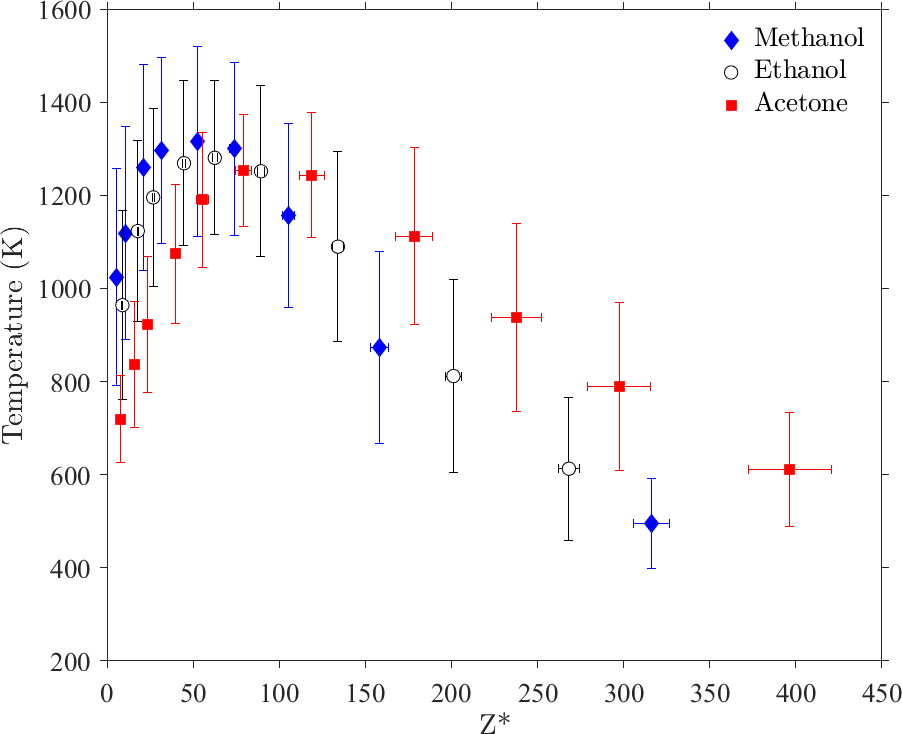
\includegraphics[width=11.0 cm, keepaspectratio]{Temperature_Comparison.png}
	\caption[Major Species Comparison]{Mean and RMS centerline temperature profiles of methanol, ethanol, and acetone pool fires during their pulsing cycles}
	\label{fig:Temp_Comparison}
\end{figure}

Figure~\ref{fig:Fuel_Comparison} displays the mean volume fraction of the major species, $\bar{X}_{i}$, as a function of $z^*$ for the methanol, ethanol, and acetone fires. Plots for individual species, including uncertainties, displayed in Appendix~\ref{sec:Vol_Frac_Figs}. Major species detected in the TCD and MSD include combustion reactants (fuels and oxygen, $\ch{O_2}$), combustion products such as water, $\ch{H_{2}O}$, and carbon dioxide, $\ch{CO_{2}}$, combustion intermediates such as carbon monoxide, $\ch{CO}$, hydrogen, $\ch{H_{2}}$, and inert gases such as nitrogen, $\ch{N_{2}}$, and argon, $\ch{Ar}$. Methane is detected and quantified in all fires. In the case of the ethanol and acetone fires, soot, benzene, acetylene, ethylene, and ethane are also detected and quantified. Trace amounts of other species are also detected including propene, acetaldehyde, and ethyl acetate, consistent with previous literature~\cite{Pichon2009, Gong2015}.

\begin{figure}[!]
	\centering
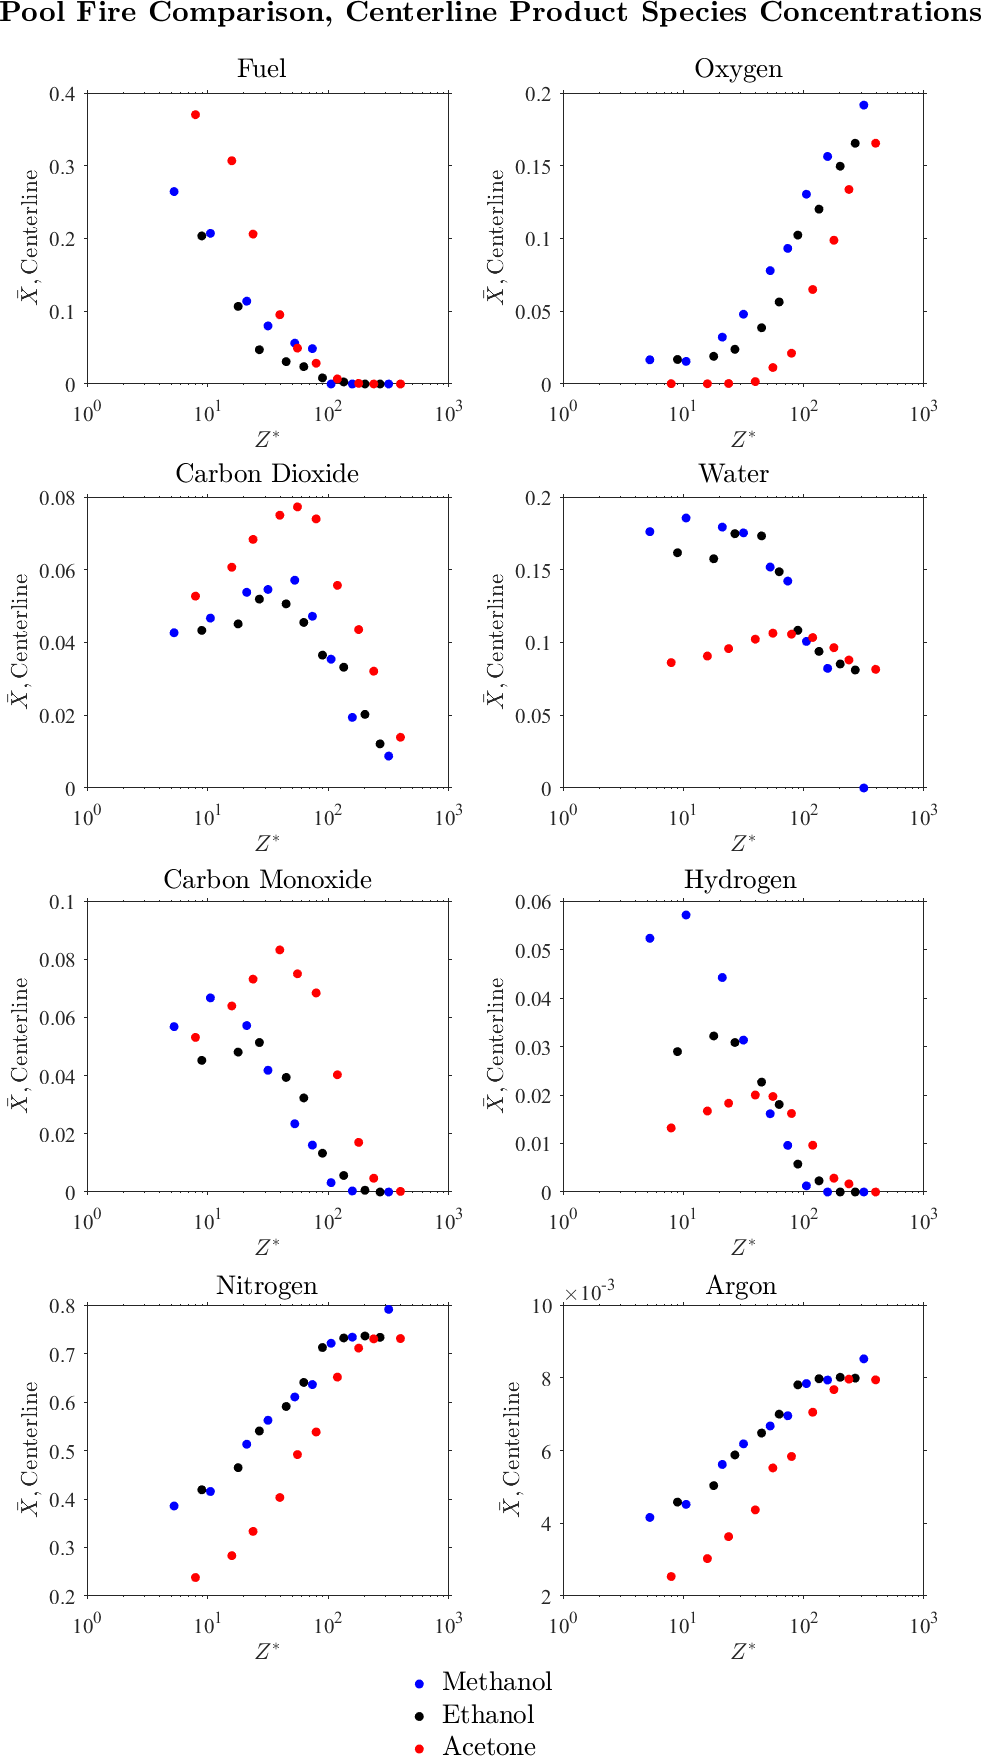
\includegraphics[width=12.5cm,keepaspectratio]{OVERALL_Fuel_Comparison.png}
	\caption[Major Species Comparison]{Centerline volume fraction and soot mass fraction profiles of methanol ($\blacklozenge$), ethanol ($\bigcirc$), and acetone ($\blacksquare$) pool fires.}
	\label{fig:Fuel_Comparison}
\end{figure}


\clearpage

\section{Verifying Gas Species Measurements}
\label{ssec:Verifying_Vol_Frac_Measurements}

This section presents several different techniques of verifying the accuracy of the species concentration measurements.


\subsection{Counting Moles}

As a way to verify the accuracy of the experimental method, specifically the calibration procedure and curve fit, the total moles, $n_{\rm tot}$, identified by the TCD and MSD is compared to the total moles injected into the GC/MSD system, $n_{\rm inj}$, which is calculated from the ideal gas law:
\begin{equation}\label{eq:moles_inj}
n_{\rm inj}=\frac{PV_{\rm s}}{RT}
\end{equation}
Here, $R=287$~J/(mol$\cdot$K) is the universal gas constant for air, $V_{\rm s}=2\times 10^{-6}$~m$^3$ is the injected sample volume, and $P$~(Pa) and $T$~(K) are the mean pressure and temperature, respectively, collected before injecting the gas sample into the GC/MSD as described in Section~\ref{ssec:Gas_Species_Setup}. The combined uncertainty of the total moles injected is detailed in Section~\ref{ssec:Total Moles Injected into the GC/MSD for Calibation}.

\begin{figure}[h!]
	\centering
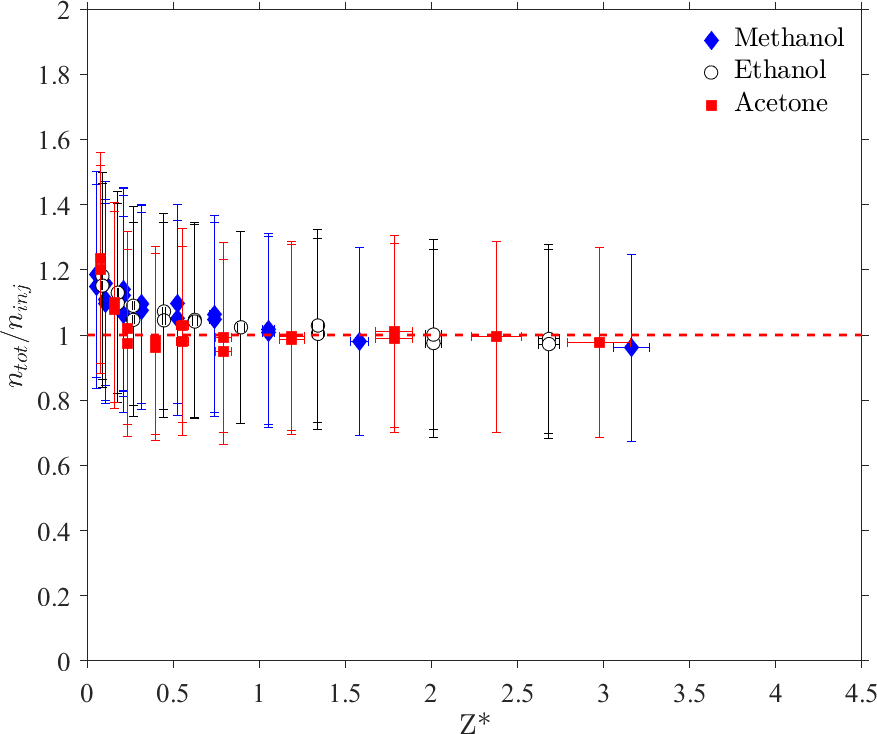
\includegraphics[width=10.5cm,keepaspectratio]{mole_ratio_Comparison.png}
	\caption[Ratio of moles identified to moles injected]{Ratio of moles identified to moles injected, with error, as a function of $z^*$}
	\label{fig:Mole_Comp}
\end{figure}

Figure~\ref{fig:Mole_Comp} shows the ratio of the moles identified by the TCD and MSD to the mole injected into the GC/MSD as a function of $z^*$. In most cases, the ratio is close to unity, indicating that the total moles injected into the GC/MS are all accounted for in the calculation. For low values of $z^*$, the ratio is higher than unity, indicating an error in the calibration which is most likely due to an over-prediction of the fuel species that are found at high concentrations near the liquid surface.

\subsection{Carbon to Hydrogen Ratio}

Another way to verify the accuracy of the gas species measurements is to calculate the ratio of carbon to hydrogen atoms contained in all gas species at each vertical measurement location:
\begin{equation}\label{eq:c2h_ratio}
  \frac{\rm C}{\rm H}=\frac{ \sum  x_i \, \bar{X}_{i} }{ \sum y_i \, \bar{X}_{i} }
\end{equation}
where the summation is over all measured gas species, and $x_i$ and $y_i$ are the numbers of carbon and hydrogen atoms in the molecule, respectively. The carbon to hydrogen ratio of the fuel molecules are reported in Table~\ref{tab:Pool_Fire_Parameters_Table}, and the ratio for each fuel is shown in Fig.~\ref{fig:C2H}.

\begin{figure}[h!]
	\centering
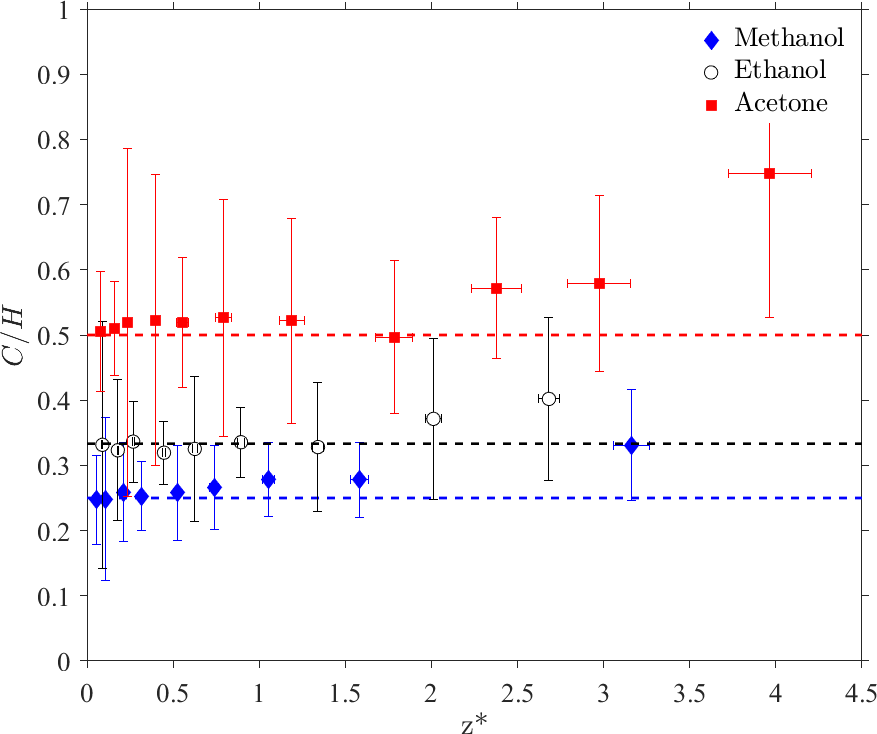
\includegraphics[width=10.5cm, keepaspectratio]{C2H_ratio_Comparison.png}
	\caption[Carbon to hydrogen ratio calculated from all species]{Carbon to hydrogen ratio calculated from all measured gas species compared to the theoretical values.}
	\label{fig:C2H}
\end{figure}

A similar verification test is to apply the summations in Eq.~(\ref{eq:c2h_ratio}) to all {\em product} species; that is, all species except the original fuel molecule. The carbon to hydrogen ratio for the product gases should be the same as that for all species. Figure~\ref{fig:SCR} shows the results. Note that an exact match is not expected because the idealized values do not take into account the mass of soot.
\begin{figure}[h!]
	\centering
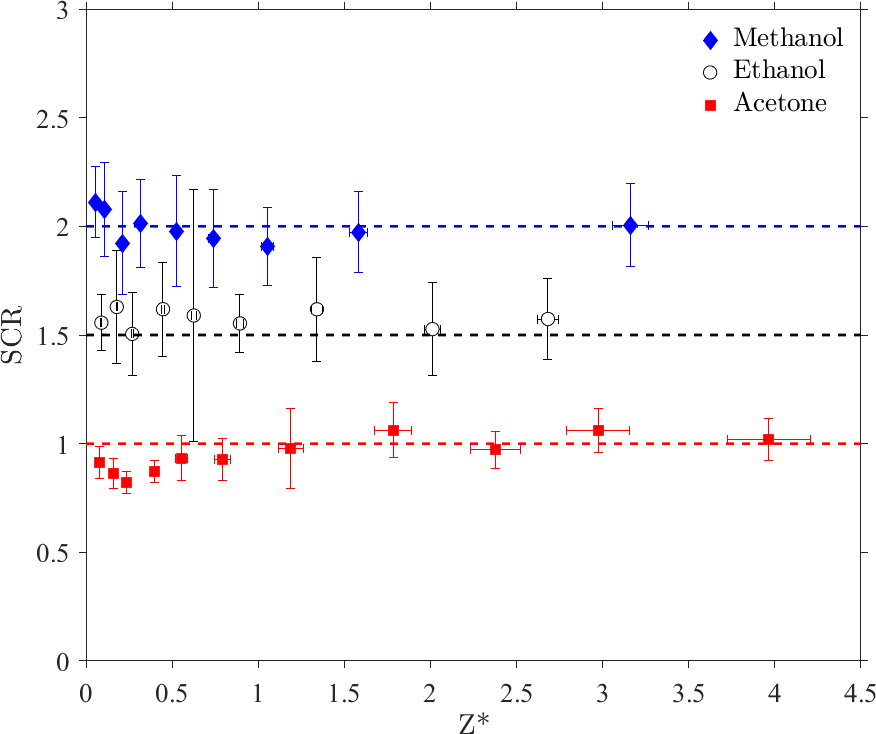
\includegraphics[width=10.5cm, keepaspectratio]{Prod_ratio_Comparison.png}
	\caption[Carbon to hydrogen ratio calculated from all {\em product} species]{Carbon to hydrogen ratio calculated from all measured {\em product} species compared to the theoretical values.}
	\label{fig:SCR}
\end{figure}

Another verification test considers the inert species argon and nitrogen whose molar ratio should be the same regardless of fuel type. The measured Ar/N$_2$ ratio in ambient air is $0.0117\pm0.0005$, and the measured ratio at different vertical locations within the fires is depicted in Fig.~\ref{fig:IR}. All points fall within the uncertainty bounds of the ambient air measurement.
\begin{figure}[h!]
	\centering
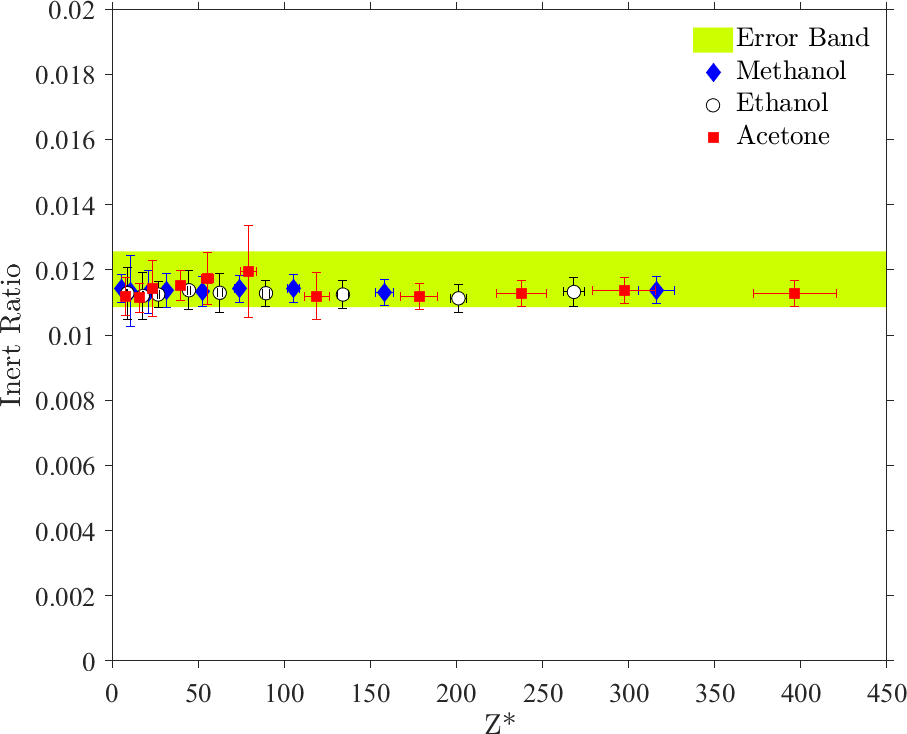
\includegraphics[width=10.5cm, keepaspectratio]{Inert_ratio_Comparison.png}
	\caption[Ar/N$_2$ ratio within the fire envelop compared to ambient air]{Ar/N$_2$ molar ratio at different elevations compared to the uncertainty bounds of the measurement in ambient air.}
	\label{fig:IR}
\end{figure}


\subsection{Plotting the Results in Mixture Fraction Space}
\label{ssec:Mixture_Fraction_Results}

The mixture fraction, $Z$, is defined as the mass fraction of the gases and soot that originate in the fuel stream. It can be expressed\footnote{The uncertainty of the mixture fraction is determined from propagating the error in the mass fraction measurements. A detailed description of the mixture fraction uncertainty is provided in Appendix~\ref{sec:Uncertainty_Mix_Frac}.} as follows:
\begin{equation}\label{eq:Mixture_Fraction}
  Z = \bar{Y}_{\rm F} + \frac{W_{\rm F}}{x} \sum_{i\ne {\rm F}} \frac{\bar{Y}_i}{W_{i}}
\end{equation}
where $\bar{Y}_{\rm F}$, ${W_{\rm F}}$, and $x$ are the mass fraction, molecular weight, and number of carbon atoms in the fuel molecule, respectively. Assuming ideal (i.e. no CO or soot), infinitely-fast (fuel and oxygen cannot co-exist) combustion, the mass fractions of all species can be expressed as piece-wise linear ``state relations'' according to the following reaction:
\begin{align*}
{\rm C}_{x}{\rm H}_{y}{\rm O}_{z} & +\eta(x+\frac{y}{4}-\frac{z}{2})~({\rm O}_{2}+3.76~{\rm N}_{2}+0.0445~{\rm Ar}) \rightarrow  \\
          & \max(0,1-\eta)~{\rm C}_{x}{\rm H}_{y}{\rm O}_{z}+\max(0,1-\eta)~(x+\frac{y}{4}-\frac{z}{2})~{\rm O}_{2}+ \min(1,\eta)~x~{\rm CO}_{2} +  \\
          & \min(1,\eta)~\frac{y}{2}~{\rm H}_{2}{\rm O}+\eta(x+\frac{y}{4}-\frac{z}{2})~(3.76~{\rm N}_{2}+0.0445~{\rm Ar})  \numberthis \label{eq:Ideal_rxn}
\end{align*}
The parameter $\eta$ is the reciprocal of the local fuel equivalence ratio, $\phi$,
\begin{equation}\label{eq:Eta}
\phi=\frac{\rm (F/A)}{{\rm (F/A)}_{\rm st}}=\frac{1}{\eta}
\end{equation}
where $\rm F/A$ is the fuel-air mass ratio and the subscript $\rm st$ denotes the stoichiometric condition.

Figures~\ref{fig:Methanol_Mix_Frac}, \ref{fig:Ethanol_Mix_Frac}, and \ref{fig:Acetone_Mix_Frac} show the mean mass fraction measurements as a function of the mixture fraction for the methanol, ethanol, and acetone fires, respectively. The dotted lines represent ideal combustion calculated from Eq.~(\ref{eq:Ideal_rxn}). The vertical dotted line identifies the stoichiometric value of the mixture fraction. Additional plots that detail the averaged mass fractions of all detected species as a function of mixture fraction, with their expanded uncertainties, are provided in Appendix~\ref{sec:Mix_Frac_Figs}.

\begin{figure}[!]
	\centering
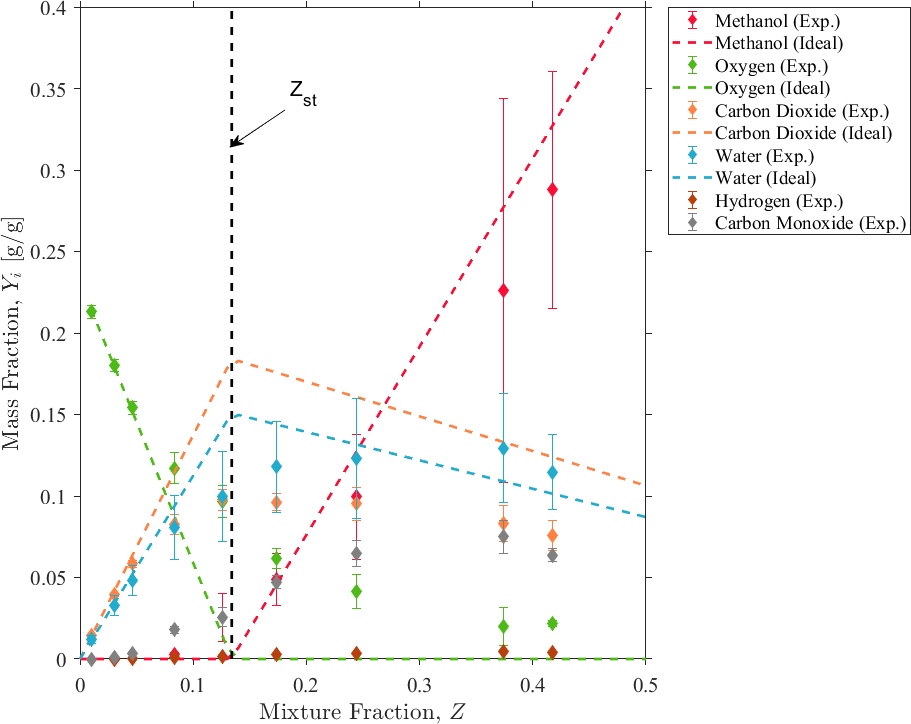
\includegraphics[width=11.0cm,keepaspectratio]{Methanol_OVERALL_Mass_Frac_Mix_Frac.png}
	\caption[Mean mass fractions as a function of mixture fraction, methanol]{Mean mass fractions as a function of mixture fraction, methanol}
	\label{fig:Methanol_Mix_Frac}
\end{figure}

\begin{figure}[!]
	\centering
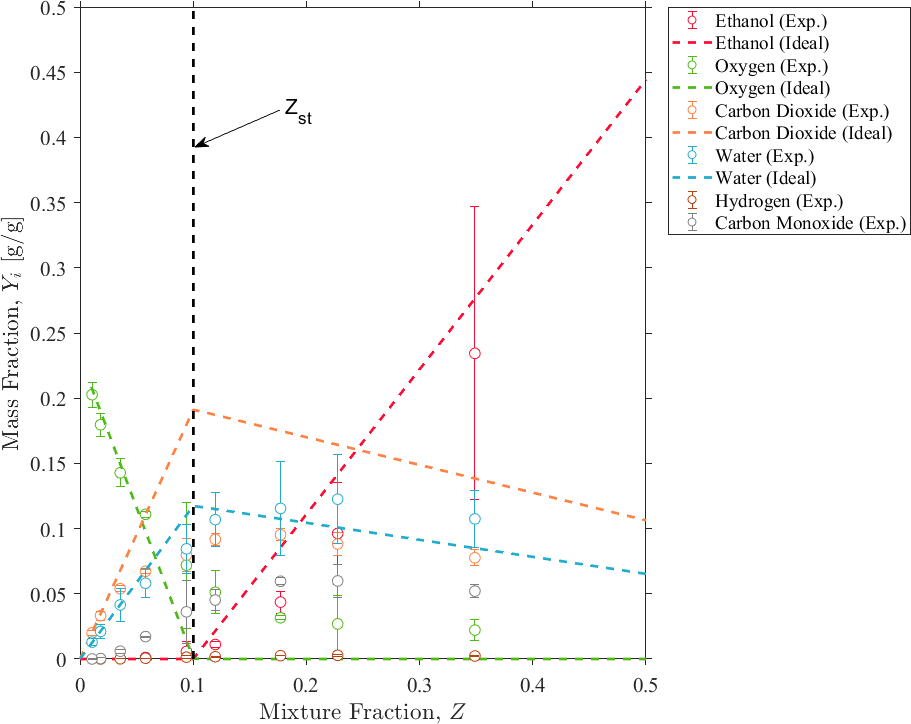
\includegraphics[width=11.0cm,keepaspectratio]{Ethanol_OVERALL_Mass_Frac_Mix_Frac.png}
	\caption[Mean mass fractions as a function of mixture fraction, ethanol]{Mean mass fractions as a function of mixture fraction, ethanol}
	\label{fig:Ethanol_Mix_Frac}
\end{figure}

\begin{figure}[!]
	\centering
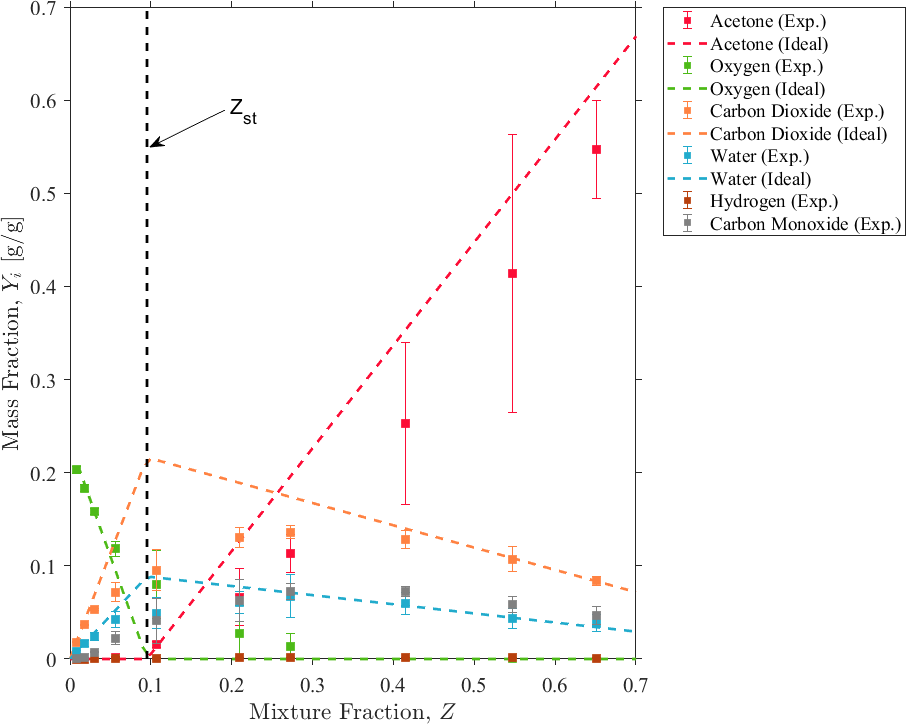
\includegraphics[width=11.0cm,keepaspectratio]{Acetone_OVERALL_Mass_Frac_Mix_Frac.png}
	\caption[Mean mass fractions as a function of mixture fraction, acetone]{Mean mass fractions as a function of mixture fraction, acetone}
	\label{fig:Acetone_Mix_Frac}
\end{figure}

Where the mixture fraction is much less than stoichiometric, all major gas species are in close agreement with the ideal state relations; the measured mass fractions of unburned fuel and $\ch{CO}$ are nearly zero, and the $\ch{O_2}$ is close to its respective theoretical value. The measured mass fraction of $\ch{CO_{2}}$ and $\ch{H_{2}O}$ are found to peak close to the stoichiometric mixture fraction. In the fuel-rich region, the measured mass fraction of $\ch{CO_{2}}$ differs considerably from the ideal state relation due to the substantial portion of $\ch{CO}$ and soot.




\clearpage

\section{Conclusion}
\label{sec:Conclusion}
In summary, time-averaged local measurements of temperature and gas species concentrations were made to characterize the structure of methanol, ethanol, and acetone \SI{30}{cm} diameter pool fire steadily burning in a quiescent environment. A verification scheme was developed to verify the gas species measurements that considered  the accuracy of the calibration and the overall stoichiometry of combustion for each fuel (see Eqn.~\ref{eq:prod_ratio_ethanol}, \ref{eq:prod_ratio_methanol}, and \ref{eq:prod_ratio_acetone}). The gas species measurements were favorably compared to the idealized SCR values, which lends confidence to the veracity of the measurements. These local measurements complement previous measurements and provide insight into the complex chemical structure of medium-scale pool fires.

\section*{Acknowledgments}
The authors would like to acknowledge Kimberly Harris of the Gas Sensing Metrology Group at NIST, who assisted in the developing the species calibration method used in the study.

\clearpage

\section*{References}
\addcontentsline{toc}{section}{References}
\bibliographystyle{techpubs}
\bibliography{References}


\clearpage


\appendix
\numberwithin{equation}{section}
\makeatletter
% "activate" the preparatory code, but for section-level headers only
\newcommand{\section@cntformat}{Appendix:\ }
\makeatother

\section{Uncertainty Analysis of Pool Fire Parameters}\label{sec:Uncertainty_Pool_Fire_Parameters}
\addcontentsline{toc}{section}{Appendix A: Uncertainty of Pool Fire Parameters}

\subsection{Mass Burning Rate}
\label{ssec:Mass_Burning_Flux}
The mass burning rate, $\dot{m}$, was measured from the mass loss in the fuel reservoir, feeding to the pool burner via gravity, during the burning period per area of the pool burner. Mass measurements were made using a Precisa XB-6200C Precision XB Laboratory Prime Balance sampling at \SI{1.0}{\hertz} for the entire duration of the burning period. The balance was calibrated from a collection standard weights. The expanded uncertainty was estimated via quadrature from a combination of the Type A and Type B evaluation of standard uncertainty. The Type A evaluation of standard uncertainty was calculated from the standard error, $s_{\scriptscriptstyle \dot{m}}$, of the time-averaged mass loss measured during the burning period. The Type B evaluation of standard uncertainty was determined from the bias error of the balance, $u_{\rm \scriptscriptstyle inst}$ (\SI{0.01}{g}), and the calibration error, $u_{\rm \scriptscriptstyle cal}$ (1~\% of the reading).

\begin{equation}
\label{eq:mass_rate_uncertainty}
u_{\scriptscriptstyle \dot{m}} = \sqrt{s_{\scriptscriptstyle \dot{m}}^2+u_{\rm \scriptscriptstyle inst}^2+u_{\rm \scriptscriptstyle cal}^2}
\end{equation}

\subsection{Heat Release Rate}
\label{ssec:Heat_Release_Rate}

The heat release rate, $\dot{Q}$, is the product of the fuel mass loss rate, $\dot{m}$, and the heat of combustion, $\Delta H$. Its uncertainty is calculated using the law of propagation of uncertainty:
\begin{equation}
\label{eq:heat_release_rate_uncertainty}
u_{\scriptscriptstyle \dot{Q}} = \sqrt{ (\Delta H \, u_{\dot{m}})^2 + (\dot{m} \, u_{\Delta H} )^2 }
\end{equation}
The description of the mass burning rate uncertainty is provided in Appendix~\ref{ssec:Mass_Burning_Flux}.

\subsection{Mean Flame Height}
\label{ssec:Mean_Flame_Height}
The mean flame height, ${L_{\rm{f}}}$, was determined by measuring the distance between the pool surface and flame tip using the photographic analysis method described in Section~\ref{ssec:Pool_Burner_Setup}. The uncertainty of the mean flame height, $u_{\scriptscriptstyle L_{\rm{f}}}$, was calculated from a combined uncertainty of the Type A and B evaluation of standard uncertainty. The Type A evaluation of standard uncertainty was estimated from the standard deviation of the height measurements, $s_{\scriptscriptstyle L_{\rm{f}}}$, made with each frame. The error of the measured distance using the photographic analysis method compared to the true distance, $u_{\scriptscriptstyle \rm{method}}$,  was found to be 0.1\% and was treated as the Type B evaluation of standard uncertainty. The combined uncertainty calculation of the mean flame height is shown below:

\begin{equation}
\label{eq:mean_flame_height}
u_{\scriptscriptstyle L_{\rm{f}}} = \sqrt{s_{\scriptscriptstyle{L_{\rm{f}}}}^2+u_{\rm \scriptscriptstyle method}^2}
\end{equation}

\pagebreak

\section{Uncertainty Analysis of Temperature Measurements}\label{sec:Uncertainty_Temperature_Measurements}
\addcontentsline{toc}{section}{Appendix B: Uncertainty of Temperature Measurements}

Temperature measurements were sampled at \SI{250.0}{Hz} for \SI{2.0}{min} using a S-type (Pt 10\% Rh/Pt), bare-wire, fine diameter thermocouple with a diameter of \SI{50.0}{\micro\metre} (OMEGA P10R-001\footref{fn:product}). Temperature measurements were corrected for following Shassix's method~\cite{Shaddix1999} and using Eqn.~\ref{eq:Thermocouple_Bead_Correction}:
\begin{equation}\label{eq:Thermocouple_Bead_Correction_full}
{T_{\rm g}(t)}= T_{\rm b}(t)+{\frac{\rho_{\rm b} \, c_{\rm b} \, {D_{\rm b}}^2}{6\, {\rm Nu} \, k_{\rm g}}}\frac{{\rm d} T_{\rm b}}{{\rm d} t}+\frac{\epsilon \, \sigma \, D_{\rm b}}{{\rm Nu} \, k_{\rm g}}\left({T_{\rm b}(t)}^4-{T_{\rm surr}(t)}^4\right)
\end{equation}
where $T_{\rm g}$ is the effective temperature of the gas, $T_{\rm surr}$ is the effective temperature of the surroundings, $k_{\rm g}$ is the thermal conductivity of the gas, $\rm Nu$ is the Nusselt number calculated from Eqn.~\ref{eq:Nu_number}, $\sigma$ is the Stefan-Boltzmann constant (\SI{5.6696E-8}{W/(m^2~K^4}), $\epsilon$ is the thermocouple emmisivity, and $T_{\rm b}$, $\rho_{\rm b}$, $c_{\rm b}$, $D_{\rm b}$ are the raw temperature measurements, density, specific heat, and diameter of the bead, respectively. The uncertainty of the effective temperature of the gas was calculated from the uncertainty of all temperature dependent parameters included in Eqn.~\ref{eq:Thermocouple_Bead_Correction_full}. The bead temperature dependent variables included in Eqn.~\ref{eq:Thermocouple_Bead_Correction_full} are $k_{\rm g}$, $\rm Nu$, $\epsilon$, $T_{\rm b}$, $\rho_{\rm b}$, $c_{\rm b}$ whereas all other parameters are considered as constant. The uncertainty of the corrected temperature measurements were estimated using a propagation of uncertainty:
 \begin{equation}
\label{eq:temperature_corr_uncer}
u_{\scriptscriptstyle T_{\rm g}} = \sqrt{{\left(\frac{\partial T_{\rm g}}{\partial T_{\rm b}}\,u_{\scriptscriptstyle T_{\rm b}} \right)}^2}
\end{equation}

\subsection{Uncertainty of Bead Temperature Measurements}
\label{ssec:Uncertain_Bead_Temp_Measurements}
The uncertainty of the raw bead temperature measurements was calculated from a combined Type A and B evaluation of uncertainty. The Type A evaluation of raw bead temperature measurements was determined from the standard error of temperature measurements, $s_{T_{\rm b}}$ from the sampling period. The Type B evaluation of uncertainty for the raw bead temperature measurements was determined from the bias error sources in the instrumentation, $u_{\rm inst}$, used to measure temperature (\SI{1.5}{\degree C}) of gas sample injected. The combined uncertainty temperature was found via quadrature:

\begin{equation}
\label{eq:temp_uncertainty}
u_{\scriptscriptstyle T_{\rm b}} = \sqrt{ u_{\rm \scriptscriptstyle inst}^2 + s_{\scriptscriptstyle T_{\rm b}}^2}
\end{equation}
\pagebreak

\section{Uncertainty Analysis of Gas Species Concentrations} \label{sec:UncertaintyGasSpecies}
\addcontentsline{toc}{section}{Appendix C: Uncertainty Analysis of Gas Species Concentrations}

\subsection{Uncertainty of Volume Fractions} \label{sec:UncertaintyMoleFrac}
As shown in Eqn.~\ref{eq:volume_fraction}, volume fraction, $\bar{X}_{i}$, was calculated from the ratio between the number of moles of a given species, $n_{i}$, and the total number of moles identified, $n_{\rm tot}$. The uncertainty of the measured volume fraction was estimated using the law of propagation of uncertainty after determining the volume fraction of each species:

\begin{equation}
\label{eq:Volume_Frac_Uncertainty}
u_\mathrm{\bar{X}_{i}} = \sqrt{{\left( \frac{\partial \bar{X}_{i}}{\partial n_{i}}\,u_{\scriptscriptstyle n_{i}} \right)}^2+{\left(\frac{\partial \bar{X}_{i}}{\partial n_{\rm tot}}\,u_{\scriptscriptstyle n_{\rm tot}}\right)}^2}
\end{equation}
A coverage factor of 2 was applied to the combined uncertainty to produce a 95~\% confidence interval.

\subsubsection{Number of Moles of a Given Species}
\label{ssec:Number_of_Moles_of_a_Given_Species}

The number of moles of a given species was determined from a calibration function of the integrated peak area of the respective species obtained from the TCD's and the MSD's Total Ion Current (TIC) chromatograms. The Type A evaluation of standard uncertainty of the number of moles of a given species was taken as the standard deviation of the measurements obtained from the repeated tests. The Type B evaluation of standard uncertainty was determined from the error in the calibration functions for each species measured by the TCD and MSD is further detailed in Appendix~\ref{sec:Uncertainty Analysis of Gas Species Calibrations}. The combined uncertainty was found via quadrature:

\begin{equation}
\label{eq:gasspeciesuncertaintycertainty}
u_{\scriptscriptstyle n_{i}} = \sqrt{ u_{\rm \scriptscriptstyle n_{i,\rm cal}}^2 + s_{\scriptscriptstyle n_{i}}^2}
\end{equation}

\subsubsection{Total Number of Moles Identified}
\label{ssec:Total Number of Moles Identified}
The total number of moles detected was determined from the summation of the number of moles for each species identified by the TCD and TIC chromatograms. Therefore, the uncertainty in the total number of moles identified was the combined uncertainty of all the identified species via quadrature:

\begin{equation}
\label{eq:totalnumberofmolesdetected}
u_{\scriptscriptstyle n_{\rm tot}}=\sqrt{{\sum_{n=1}^{N} s_{\scriptscriptstyle n_{i}}^2}}
\end{equation}
where $N$ is the number of a species identified species in the TCD and TIC chromatogram.

\subsection{Uncertainty of Mass Fractions}
\label{ssec:Uncertainty of Mass Fractions}
Mass fraction of a given species was calculated using its measured volume fraction, $\bar{X_{i}}$, molecular weight, $W_i$ , and the average molecular weight of all detected gas species, $W_{\rm tot}$, as shown in Eqn.~\ref{eq:mass_fraction}. The uncertainty of the mass fraction of a given species was estimated from the law of propagation of uncertainty using Eqn.~\ref{eq:mass_fraction}.
\begin{equation}\label{eq:Mass_Frac_Uncertainty}
u_\mathrm{\bar{Y}_{i}} = \sqrt{{\left( \frac{\partial \bar{Y}_{i}}{\partial \bar{X}_{i}}\,u_{\scriptscriptstyle \bar{X}_{i}} \right)}^2+{\left(\frac{\partial \bar{Y}_{i}}{\partial W_{\rm tot}}\,u_{\scriptscriptstyle W_{tot}}\right)}^2}
\end{equation}

\subsubsection{Uncertainty of the average molecular weight}
\label{ssec:Uncertainty of the average molecular weight}
The uncertainty of the average molecular weight was determined using the law of propagation of uncertainty, which accounted for each detected species measured from the injected sample.

\begin{equation}\label{eq:Uncertainty_Total_MW}
	u_{\scriptscriptstyle W_{tot}}=\sqrt{\left(\sum{{u_{\scriptscriptstyle \bar{X}_{i}}}{{W_{i}}}}\right)^2}
\end{equation}

\pagebreak

\section{Uncertainty Analysis of Gas Species Calibrations}\label{sec:Uncertainty Analysis of Gas Species Calibrations}
\addcontentsline{toc}{section}{Appendix D: Uncertainty Analysis of Gas Species Calibrations}
A calibration function is a relationship between an integrated peak area on the TCD or TIC chromatogram, $\rm{Area}_{i}$, and the number of moles of a given species injected into the GC/MSD, $n_{i}$. A calibration function was determined by injecting a known amount of moles of a given species into the GC/MSD, $n_{i,\rm cal}$, and identifying the peak area corresponding to the individual species. For this work, the calibration functions are approximately linear consisting of a slope, $a$, and intercept, $b$.

\begin{equation}
\label{eq:Calibration Curve}
n_{i,\rm cal} = a \, (\rm {Area}_{i})+b
\end{equation}

Calibration functions were weighted to account for the error of each gas standard used in the calibration procedure. The uncertainty of a calibration function was determined using the law of propagation of uncertainty:

\begin{equation}
\label{eq:Given_Moles_Uncertainty}
 u_{\rm \scriptscriptstyle n_{i}} = \sqrt{{\left( \frac{\partial n_{i}}{\partial a}\,u_{\scriptscriptstyle a} \right)}^2+{\left(\frac{\partial {n_{i}}}{\partial b}\,u_{\scriptscriptstyle b}\right)}^2}
\end{equation}
The uncertainties of the slope and intercept in a weighting linear regression are as follows:
\begin{equation}
\label{eq:Slope_Uncertainty}
u_{\rm \scriptscriptstyle a} =\sqrt{\frac{\sum~\frac{1}{u_{n_{i,\rm cal}}}}{(\sum~\frac{\rm{Area}_{i}^2}{{u_{n_{i,\rm cal}}^2}})(\sum~\frac{1}{{u_{n_{i,\rm cal}}^2}})-(\sum~\frac{\rm{Area}_{i}}{{u_{n_{i,\rm cal}}^2}})^2}}
\end{equation}
\begin{equation}
\label{eq:Intercept_Uncertainty}
u_{\rm \scriptscriptstyle b} =\sqrt{\frac{\sum~\frac{\rm{Area}_{i}^2}{u_{n_{i,\rm cal}}}}{(\sum~\frac{\rm{Area}_{i}^2}{{u_{n_{i,\rm cal}}^2}})(\sum~\frac{1}{{u_{n_{i,\rm cal}}^2}})-(\sum~\frac{\rm{Area}_{i}}{{u_{n_{i,\rm cal}}^2}})^2}}
\end{equation}
where $u_{n_{i,\rm cal}}$ is the uncertainty of the known number of moles of the respective species.

During calibration, the number of moles of a given species $n_{i,\rm cal}$ was calculated from the product of the total moles injected into the GC/MSD, $n_{\rm inj}$, and the known concentration of the particular species in the calibration standard, $C_{i}$.

\begin{equation}
\label{eq:Cal_Moles}
n_{i,\rm cal} = C_{i}(n_{\rm inj})
\end{equation}
A collection of gas calibration standards for a variety of species were pre-selected to provide a broad range of concentrations. All calibration standards were mixtures of the target gas species with a Nitrogen balance, with the exception of one standard balanced in Air. A list of gas standards used in this work, with their respective concentrations and Type B evaluation of standard uncertainty, is provided in Appendix~\ref{sssec:Table of Gas Standards with Error}.

The uncertainty of the number of moles of a given species injected into the GC/MSD for calibration was estimated using the law of propagation of uncertainty:

\begin{equation}
\label{eq:Given_Moles_Cal_Uncertainty}
 u_{\rm \scriptscriptstyle n_{i,\rm cal}} = \sqrt{{\left( \frac{\partial n_{i,\rm cal}}{\partial C_{i}}\,u_{\scriptscriptstyle C_{i}} \right)}^2+{\left(\frac{\partial n_{i,\rm cal}}{\partial n_{\rm inj}}\,u_{\scriptscriptstyle n_{\rm inj}}\right)}^2}
\end{equation}

\subsection{Total Moles Injected into the GC/MSD for Calibation}
\label{ssec:Total Moles Injected into the GC/MSD for Calibation}

The total moles injected into the GC/MSD, $ n_{\rm inj}$, for calibration was determined from Eq/~\ref{eq:moles_inj} using the pressure, $P$, temperature, $T$, and volume, $V_{\rm s}$, of the gas sample injected into the GC/MSD. Pressure and temperature measurements were made using a digital pressure gauge (OMEGA P10R-001\footref{fn:product}) and K-type thermocouple located at the GC/MSD sample loop injection valve, respectively, sampling at \SI{2}{Hz} for \SI{50}{s}. The volume of the GC/MSD sample loop was \SI{2}{ml}. The Type A evaluation of uncertainty of the total moles injected into the GC/MSD for calibration was determined from the standard error of the pressure, $s_{P}$, and temperature, $s_{T}$ readings from the sampling period. The Type B evaluation of uncertainty for the total moles injected into the GC/MSD for calibration was determined from the bias error sources in the instrumentation, $u_{\rm inst}$, used to measure pressure (0.008\% accuracy of the reading) and temperature (\SI{1.5}{\degree C}) of gas sample injected. The combined uncertainty of the pressure and temperature was found via quadrature:

\begin{equation}
\label{eq:pressure_uncertainty}
u_{\scriptscriptstyle P} = \sqrt{ u_{\rm \scriptscriptstyle inst}^2 + s_{\scriptscriptstyle P}^2}
\end{equation}
\begin{equation}
\label{eq:temp_uncertainty}
u_{\scriptscriptstyle T} = \sqrt{ u_{\rm \scriptscriptstyle inst}^2 + s_{\scriptscriptstyle T}^2}
\end{equation}
The standard uncertainty of the total moles injected into the GC/MSD for calibration was estimated using the law of propagation of uncertainty:
\begin{equation}
\label{eq:moles_injected_uncertainty}
u_{\scriptscriptstyle n_{\rm inj}} = \sqrt{{\left( \frac{\partial n_{\rm inj}}{\partial P}\,u_{\scriptscriptstyle P} \right) }^2+{\left(\frac{\partial n_{\rm inj}}{\partial T}\,u_{\scriptscriptstyle T}\right)}^2}
\end{equation}

\pagebreak
\subsection{Table of Gas Standards with Error}
\label{sssec:Table of Gas Standards with Error}
A table of the gas standards with their respective concentrations and Type B evaluation of standard uncertainty, used for calibrating the GC/MSD is provided below. Lot numbers for all standards are provided for traceability.

\begin{table}[h!]

\caption{Gas Standards used to Calibrate GC/MSD}
\label{tab:Gas_Standards_Table}
\centering
	\footnotesize
	\begin{tabular}{lcll}
			\hline
%\\[0.0005cm]
\textbf{Components} &\textbf{Uncertainty(\%)}& \textbf{Distributor}	& \textbf{Lot No.}		\\
\hline
\\[0.001cm]
200 ppm Acetone		&	2.00	&	Gasco Affiliates, LLC. 				&	DNJ-ACE-200N-1		\\
0.26\% Acetylene		&	2.00	&	Gasco Affiliates, LLC.				&	FBJ-M24-0.25\%-1		\\
1.04\% Acetylene		&	2.00	&	Gasco Affiliates, LLC.				&	FBJ-M24-1			\\
1.02\% Argon		&	2.00	&	Gasco Affiliates, LLC.				&	DBJ-2-1N-1			\\
88.5\% Argon		&	2.00	&	Gasco Affiliates, LLC.				&	DBJ-2-90N-1			\\
100 ppm Benzene		&	2.00	&	Gasco Affiliates, LLC.				&	FBJ-21-100-3		\\
15.6\% Carbon Dioxide	&	0.04	&	NIST Gas Sensing Metrology Group		&	9-C-44			\\
24.5\% Carbon Dioxide	&	2.00	&	Gasco Affiliates, LLC. 				&	KBI-35-25-1			\\
1.00\% Carbon Dioxide	&	2.00	&	Matheson Tri-Gas					&	9306620888			\\
2.51\% Carbon Dioxide	&	2.00	&	Roberts Oxygen					&	1002080917			\\
7.00\% Carbon Dioxide	&	2.00	&	Roberts Oxygen					&	1009010318			\\
0.30\% Carbon Monoxide	&	2.00	&	Roberts Oxygen					&	1009010318			\\
9.00\% Carbon Dioxide	&	2.00	&	Praxair Doistribution Inc. 				&	304113044702		\\
0.02\% Carbon Monoxide	&	2.00	&	Matheson Tri-Gas					&	9306620888			\\
0.11\% Carbon Monoxide	&	2.00	&	Roberts Oxygen					&	1002080917			\\
4.00\% Carbon Monoxide	&	2.00	&	Praxair Doistribution Inc. 				&	304113044702		\\
7.81\% Carbon Monoxide	&	0.02	&	NIST Gas Sensing Metrology Group 		&	51-28-C			\\
0.51\% Ethane		&	2.00	&	Gasco Affiliates, LLC.				&	FBJ-62N-0.5-1		\\
1.00\% Ethane		&	2.00	&	Gasco Affiliates, LLC.				&	FBJ-152N-1-1\%-1		\\
2.55\% Ethane		&	2.00	&	Gasco Affiliates, LLC.				&	FBJ-152N-2.5-1		\\
0.51\% Ethylene		&	2.00	&	Gasco Affiliates, LLC.				&	FBJ-62N-0.5\%-1		\\
1.02\% Ethylene		&	2.00	&	Gasco Affiliates, LLC.				&	FBJ-62N-1\%-1		\\
2.55\% Ethylene		&	2.00	&	Gasco Affiliates, LLC.				&	FBJ-62N-2.5\%-1		\\
0.26\% Hydrogen		&	2.00	&	Gasco Affiliates, LLC.				&	FBJ-84-0.25-1		\\
0.50\% Hydrogen		&	2.00	&	Gasco Affiliates, LLC.				&	KBI-84-0.5-1			\\
1.00\% Hydrogen		&	2.00	&	Gasco Affiliates, LLC.				&	KBI-84-1-3			\\
2.00\% Hydrogen		&	2.00	&	Gasco Affiliates, LLC.				&	FBJ-84-2-5			\\
4.03\% Hydrogen		&	2.00	&	Gasco Affiliates, LLC.				&	FBJ-84-4-2			\\
0.40\% Methane		&	2.00	&	Gasco Affiliates, LLC. 				&	DBJ-135N-0.4-1		\\
3.95\% Methane		&	2.00	&	Gasco Affiliates, LLC.				&	DBJ-135N-4-2		\\
40.8\% Methane		&	2.00	&	Gasco Affiliates, LLC.				&	DBJ-135N-40-1		\\
0.50\% Oxygen		&	2.00	&	Gasco Affiliates, LLC. 				&	DBJ-2-90N-1			\\
1.97\% Oxygen		&	0.01	&	NIST Gas Sensing Metrology Group		&	73-D-03			\\
5.02\% Oxygen		&	2.00	&	Gasco Affiliates, LLC.				&	DBJ-161-5-5			\\
9.92\% Oxygen		&	0.02	&	NIST Gas Sensing Metrology Group		&	72-D-60			\\
10.2\% Oxygen		&	2.00	&	Gasco Affiliates, LLC. 				&	KBI-161-10-6		\\
20.7\% Oxygen		&	0.04	&	NIST Gas Sensing Metrology Group		&	71-D-51			\\
0.42\% Propane		&	2.00	&	Gasco Affiliates, LLC.				&	DBJ-176N-0.4-1		\\
39.6\% Propane		&	2.00	&	Gasco Affiliates, LLC. 				&	DBJ-176N-40-1		\\
%\\[0.005cm]
\hline
\end{tabular}
\end{table}

\pagebreak
\subsection{Concentration of Vapors from Bubblers}
\label{sssec:Concentration of Vapors from Bubblers}

Liquid material concentrations were calibrated from the ratio of the liquid-vapor pressure to the total pressure injected into the GC/MSD.

\begin{equation}
\label{eq:liquid_vapor_concentration}
C_{\rm vap} =\frac {P_{\rm vap}}{P}
\end{equation}

The vapor pressure of any given liquid can be calculated and modified using the bubbler setup shown in Fig.~\ref{fig:Bubbler}:

\begin{figure}[h!]
	\centering
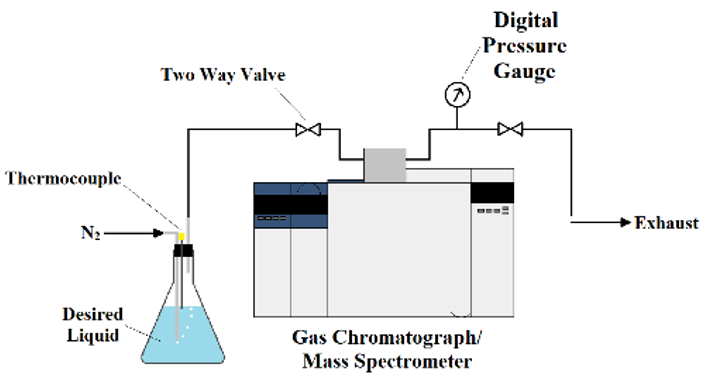
\includegraphics[width=\textwidth,keepaspectratio]{Bubbler_Setup.png}
	\caption[Flow diagram for bubble calibration system used for liquid materials]{Flow diagram for bubble calibration system used for liquid materials (acetone, ethanol, methanol, and water)}
	\label{fig:Bubbler}
\end{figure}
Nitrogen, acting as a carrier gas, was bubbled at the bottom of a liquid bath which after reaching the liquid surface transport vapor molecules through a heated gas line and into the GC/MSD sample loop. The concentration of the vapor injected into the GC/MSD was calculated from a liquid-vapor pressure correlation provided by DIPPR\textsuperscript{\textregistered}.

\begin{equation}
\label{eq:liquid_vapor_pressure_correlation}
P_{\rm vap} ={\rm e}^{A+\frac{B}{T_{\rm B}}+C\,\ln{(T_{\rm B})}+D\,(T_{B})^{E}}
\end{equation}
In this correlation, $P_{\rm vap}$ is the vapor pressure calculated from the temperature of the liquid bath, $T_{\rm B}$, with the coefficients ($A$, $B$, $C$, $D$, $E$) specific to the liquid material. Table~\ref{tab:Liquid Calibrate_Table} lists all coefficients for each calibrated liquid, including the uncertainty of their respective correlations, $u_{\rm corr}$.

\begin{table}[!]
\caption{Liquid Vapor Pressure Correlation Coefficients for Various Calibrated Liquids}
\label{tab:Liquid Calibrate_Table}
\centering
	\footnotesize
	\begin{tabular}{lcccccc}
			\hline
%\\[0.0005cm]
\textbf{Liquid Material} &\textbf{A}& \textbf{B}& \textbf{C}&\textbf{D}&\textbf{E}&\textbf{Uncertainty(\%)}\\
\hline
\\[0.001cm]
Acetone	&	69.006	&	-5599.6	&	-7.0985	&	6.2237E-6	& 	2.00	&  3.00\\
Ethanol	&	73.304	&	-7122.3	&	-7.1424	&	2.8853E-6	& 	2.00	&  1.00\\
Methanol	&	82.718	&	-6904.5	&	-8.8622	&	7.4664E-6	& 	2.00	&  3.00\\
Water		&	73.649	&	-7258.2	&	-7.3037	&	4.1653E-6	& 	2.00	&  0.20\\
%\\[0.01cm]
\hline
\end{tabular}
\end{table}

The concentration range of each calibrated liquid typically spanned between 2~\% and 50~\%. Liquid bath temperatures were controlled using a heating plate positioned underneath the insulated bubbler. The temperature of the bath was measured using a K-type thermocouple placed at the liquid bath's surface. The liquid bath temperature measurements were sampled at \SI{2.0}{\hertz} for \SI{50}{s} simultaneously with pressure and temperature measurements of the GC/MSD sample loop. Liquid-vapor calibrations were conducted once the bath a steady-state temperature (approximately 1 hour) and the Nitrogen/vapor gas mixture has swept through the GC/MSD sample loop. Upon injection into the GC/MSD, pressure and temperature measurements of the sample loop are made as previously describe in Appendix~\ref{ssec:Total Moles Injected into the GC/MSD for Calibation}.

The uncertainty of the concentration determined using Eqn.~\ref{eq:liquid_vapor_concentration} was estimated using the law of propagation of uncertainty:
\begin{equation}
\label{eq:vapor_concentration_uncertainty}
u_{\scriptscriptstyle C_{\rm vap}} = \sqrt{{\left( \frac{\partial C_{\rm vap}}{\partial P}\,u_{\scriptscriptstyle P} \right) }^2+{\left(\frac{\partial C_{\rm vap}}{\partial P_{\rm vap}}\,u_{\scriptscriptstyle P_{\rm vap}}\right)}^2}
\end{equation}

The uncertainty of the pressure measured upon injected was calculated from Eqn.~\ref{eq:pressure_uncertainty}. The uncertainty of the vapor pressure was found by combining the propagated error of liquid bath temperauture and the uncertainty in the correlation via quadrature:

\begin{equation}
\label{eq:vapor_concentration_uncertainty}
u_{\scriptscriptstyle P_{\rm vap}} = \sqrt{{\left(\frac{\partial P_{\rm vap}}{\partial T_{\rm B}}\,u_{\scriptscriptstyle T_{\rm B}} \right)}^2+{u_{\rm corr}}^2}
\end{equation}

The Type A evaluation of uncertainty of the liquid bath temperautre readings was determined from the standard error of the temperature, $s_{T_{\rm B}}$ readings from the sampling period. The Type B evaluation of uncertainty for the liquid bath temperature was defined as the bias error source (\SI{1.5}{\degree C}) in the thermocouple, $u_{\rm inst}$. The combined uncertainty liquid bath temperature was determined via quadrature:

\begin{equation}
\label{eq:temp_bath_uncertainty}
u_{\scriptscriptstyle T_{B}} = \sqrt{u_{\rm \scriptscriptstyle inst}^2 + s_{\scriptscriptstyle T_{\rm B}}^2}
\end{equation}
\pagebreak

\section{Uncertainty Analysis of the Soot Mass Fraction} \label{sec:Uncertainty_Soot_Frac}
\addcontentsline{toc}{section}{Appendix E: Uncertainty Analysis of the Soot Mass Fraction}
The local soot mass fraction measurements, $M_{\rm s}$ made at various heights above the fuel surface in pool fires of different fuels were calculated through a combination of Eqns.~\ref{eq:soot_mass_frac}, \ref{eq:total_mass}, and \ref{eq:gas_density}:
\begin{equation}\label{eq:overall_soot_mass_frac}
Y_{\rm s}= \frac{m_{\rm s} \, V_{s}}{\dot{V} \, t \, m_{\rm tot}}\frac{T_{\rm \infty}}{T_{\rm g}}
\end{equation}
where $m_{\rm s}$ is the mass of soot collected on the PTFE filter and gun cleaning patches, $\dot{V}$ is the volumetric flow rate measured by the mass flow controller, $V_{s}$ is the volume of the sample loop, $m_{\rm tot}$ is the total mass of the gas sample detected in the TCD and TIC chromatograms calculated from the summation of the product of the number of moles of a given species and their respective molar mass, $T_{\rm \infty}/T_{\rm g}$ is the ratio of the internal gas flow temperature readings of the mass flow controller to the temperature of the probe, and $t$ is the total sampling time. The uncertainty of the measured soot mass fraction was estimated using the law of propagation of uncertainty after determing the soot mass fraction:

\begin{equation}
\label{eq:soot_mass_frac_uncertainty}
u_{\scriptscriptstyle Y_{\rm s}} = \sqrt{{\left(\frac{\partial Y_{\rm s}}{\partial m_{\rm s}}\,u_{\scriptscriptstyle m_{\rm s}} \right)}^2+{\left(\frac{\partial Y_{\rm s}}{\partial \dot{V} }\,u_{\scriptscriptstyle \dot{V}} \right)}^2+{\left(\frac{\partial Y_{\rm s}}{\partial m_{\rm tot}}\,u_{\scriptscriptstyle m_{\rm tot}} \right)}^2+{\left(\frac{\partial Y_{\rm s}}{\partial T_{\rm \infty}}\,u_{\scriptscriptstyle T_{\rm \infty}} \right)}^2+{\left(\frac{\partial Y_{\rm s}}{\partial T_{\rm g}}\,u_{\scriptscriptstyle T_{\rm g}} \right)}^2}
\end{equation}
A coverage factor of 2 was applied to the combined uncertainty to produce a 95~\% confidence interval.

\subsection{Mass of Soot}
\label{ssec:Mass_of_Soot}

The mass of soot was measured from the difference in mass of a dried PTFE filter and dried gun cleaning patches immediately before and \SI{48}{hrs} after each test. The Type A evaluation of standard uncertainty of the mass of soot, $m_{\rm s}$ was taken as the standard deviation, $s_{m_{\rm s}}$, of the measurements sampled three times before and after each test. The Type B evaluation of uncertainty, $u_{\rm inst}$, was determined from the instrumentation error sources of the scale and was found to be 1~\% of the reading. The combined uncertainty was found via quadrature:

\begin{equation}
\label{eq:soot_mass_uncertainty}
u_{\scriptscriptstyle m_{\rm s}} = \sqrt{u_{\rm \scriptscriptstyle inst}^2 + s_{\scriptscriptstyle m_{\rm s}}^2}
\end{equation}

\subsection{Mass Flow Controller Volumetric Flow Rate}
\label{ssec:Mass_Flow_Controller_Volumetric_Flow_Rate}

A mass flow controller was used to measure the volumetric flow rate, $\dot{V}$, within the gas sampling line. The Type A evaluation of standard uncertainty was taken as the standard deviation of the flow measurements sampled at \SI{2}{Hz} during the gas sampling period which varied from\SI{12}{min} to \SI{25}{min} depending on the sampling location within the fire. The Type B evaluation of standard uncertainty was determined from the calibration error, $u_{\rm cal}$, and the precision error sources at calibration conditions, $u_{\rm p.e.}$, defined as \SI{2}{ml} and 0.8~\% of the reading + 0.2~\% of the full scale (\SI{2}{L/min}), respectively. The combined uncertainty was calculated via quadrature:

\begin{equation}
\label{eq:volumetric_flow_uncertainty}
u_{\scriptscriptstyle \dot{V}} = \sqrt{u_{\rm \scriptscriptstyle p.e.}^2 + u_{\rm \scriptscriptstyle cal}^2 + s_{\scriptscriptstyle \dot{V}}^2}
\end{equation}

\subsection{Total Mass Identified}
\label{ssec:Total_Mass_Identified_into_GC/MSD}
The total mass detected in the TCD and TIC chromatograms, $m_{\rm tot}$, was calculated from the summation of products of the number moles of a given species that were identified from the TCD and TIC chromatograms, $n_{i}$, and their respective molar mass, ${\textrm{W}_{i}}$:

\begin{equation}
\label{eq:total_mass_detected_uncertainty}
m_{\rm tot}=\sum_{n=1}^{N} n_{i}{\textrm{W}_{i}}
\end{equation}

The uncertainty in the total mass detected was calculated from the uncertainties of all identified species, defined in Section~\ref{ssec:Total Number of Moles Identified}, multiplied by their corresponding molar mass via quadrature:

\begin{equation}
\label{eq:total_mass_detected_uncertainty}
u_{\scriptscriptstyle m_{\rm tot}}=\sqrt{{\sum_{n=1}^{N} (u_{\scriptscriptstyle n_{i}}{\textrm{W}_{i}})^2}}
\end{equation}
where $N$ is the number of a species identified species in the TCD and TIC chromatograms.

\subsection{Mass Flow Controller Internal Gas Flow Temperature Reading}
\label{ssec:MFC_Temp}

The mass flow controller provides an internal gas flow temperature reading that was recorded manually during the gas sampling process. The uncertainty of the temperature reading was determined from the Type B evaluation of standard uncertainty of the mass flow controller temperature measurement defined as 0.75~\% of the reading.

\subsection{The Effective Temperature of the Gas}
\label{ssec:Probe_Temp}

The uncertainty of the temperature measurements at the entrance of the probe is described in Appendix~\ref{sec:Uncertainty_Temperature_Measurements}.

\pagebreak

\section{Uncertainty Analysis of the Mixture Fraction}\label{sec:Uncertainty_Mix_Frac}
\addcontentsline{toc}{section}{Appendix F: Uncertainty of the Mixture Fraction}
The mixture fraction, $Z$, was determined from Eqn.~\ref{eq:Mixture_Fraction} based on carbon containing species. The uncertainty of the determined mixture fraction was estimated from the law of propagation of uncertainty using mass fractions of carbon containing species, $\bar{Y}_{i,c}$, and the parent fuel, $\bar{Y}_{f}$.
\begin{equation}
\label{eq:mixture_frac_uncertainty}
u_{\scriptscriptstyle Z}=\sqrt{{u_{\scriptscriptstyle \bar{Y}_{f}}}^2+{\sum_{i=1}^{N}{\left(\frac{\partial Z}{\partial \bar{Y}_{i,C}}\frac{u_{\scriptscriptstyle \bar{Y}_{i,C}}}{\textrm{W}_{i}} \right)}^2}}
\end{equation}
The uncertainty of the mass fractions of carbon containing species is discussed in Appendix~\ref{ssec:Uncertainty of Mass Fractions}.

\pagebreak

\section{Uncertainty Analysis of the $Z^{*}$}\label{sec:Uncertainty_Z_star}
\addcontentsline{toc}{section}{Appendix H: Uncertainty Analysis of the $Z^{*}$}
$Z^{*}$ was calculated from Eqn.~\ref{eq:Z_Star} where the gravitational constant and temperature, specific heat, and density of the ambient air were treated as constants. The uncertainty of $Z^{*}$ was calculated from the law of propagation of uncertainty, which incorporated the uncertainties of the heat release rate, $\dot{Q}$, and the mean flame height, $L_{\rm{f}}$.
\begin{equation}
\label{eq:heat_release_rate_uncertainty}
u_{\scriptscriptstyle Z^{*}} = \sqrt{{\left(\frac{\partial Z^{*}}{\partial \dot{Q}}\,u_{\scriptscriptstyle \dot{Q}} \right)}^2+{\left(\frac{\partial Z^{*}}{\partial L_{\rm{f}}}\,u_{\scriptscriptstyle L_{\rm{f}}} \right)}^2}
\end{equation}
The uncertainty of the heat release rate and mean flame height is described in Appendix~\ref{sec:Uncertainty_Pool_Fire_Parameters}.

\pagebreak

\section{Figures of Averaged Volume Fractions of Centerline Measurements as a Function of $Z^{*}$ for Methanol, Ethanol, and Acetone Fires}\label{sec:Vol_Frac_Figs}
\addcontentsline{toc}{section}{Appendix H: Figures of Averaged Volume Fractions of Centerline Measurements as a Function of $Z^{*}$ for Methanol, Ethanol, and Acetone Fires}

\subsection{Methanol}
\label{ssec:Methanol_ALL_Vol_Frac}
\begin{figure}[!h]
	\centering
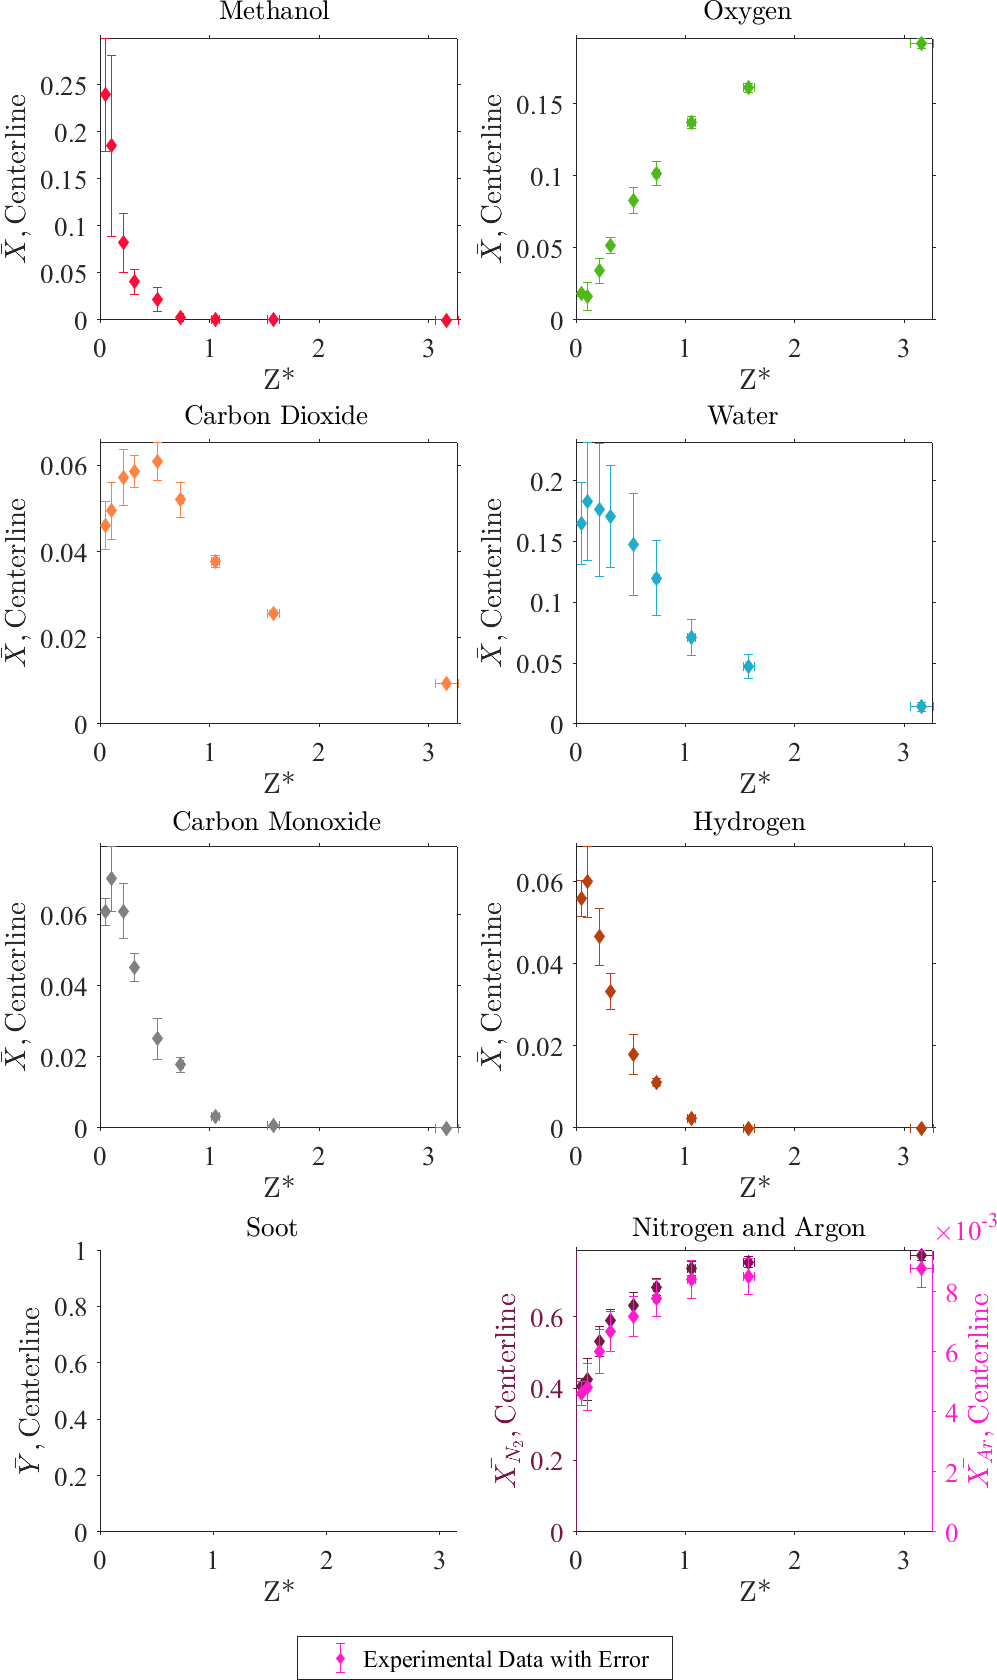
\includegraphics[width=10.0cm,keepaspectratio]{Methanol_MOL_FRAC_Plot.png}
	\caption[Plot of volume fractions, with error, of major species identified in the methanol pool fire centerline as function of $Z^{*}$]{Plot of volume fractions of major species identified in the methanol pool fire centerline as function of $Z^{*}$}
	\label{fig:Methanol_VOL_Frac_Major}
\end{figure}
\pagebreak

\begin{figure}[!h]
	\centering
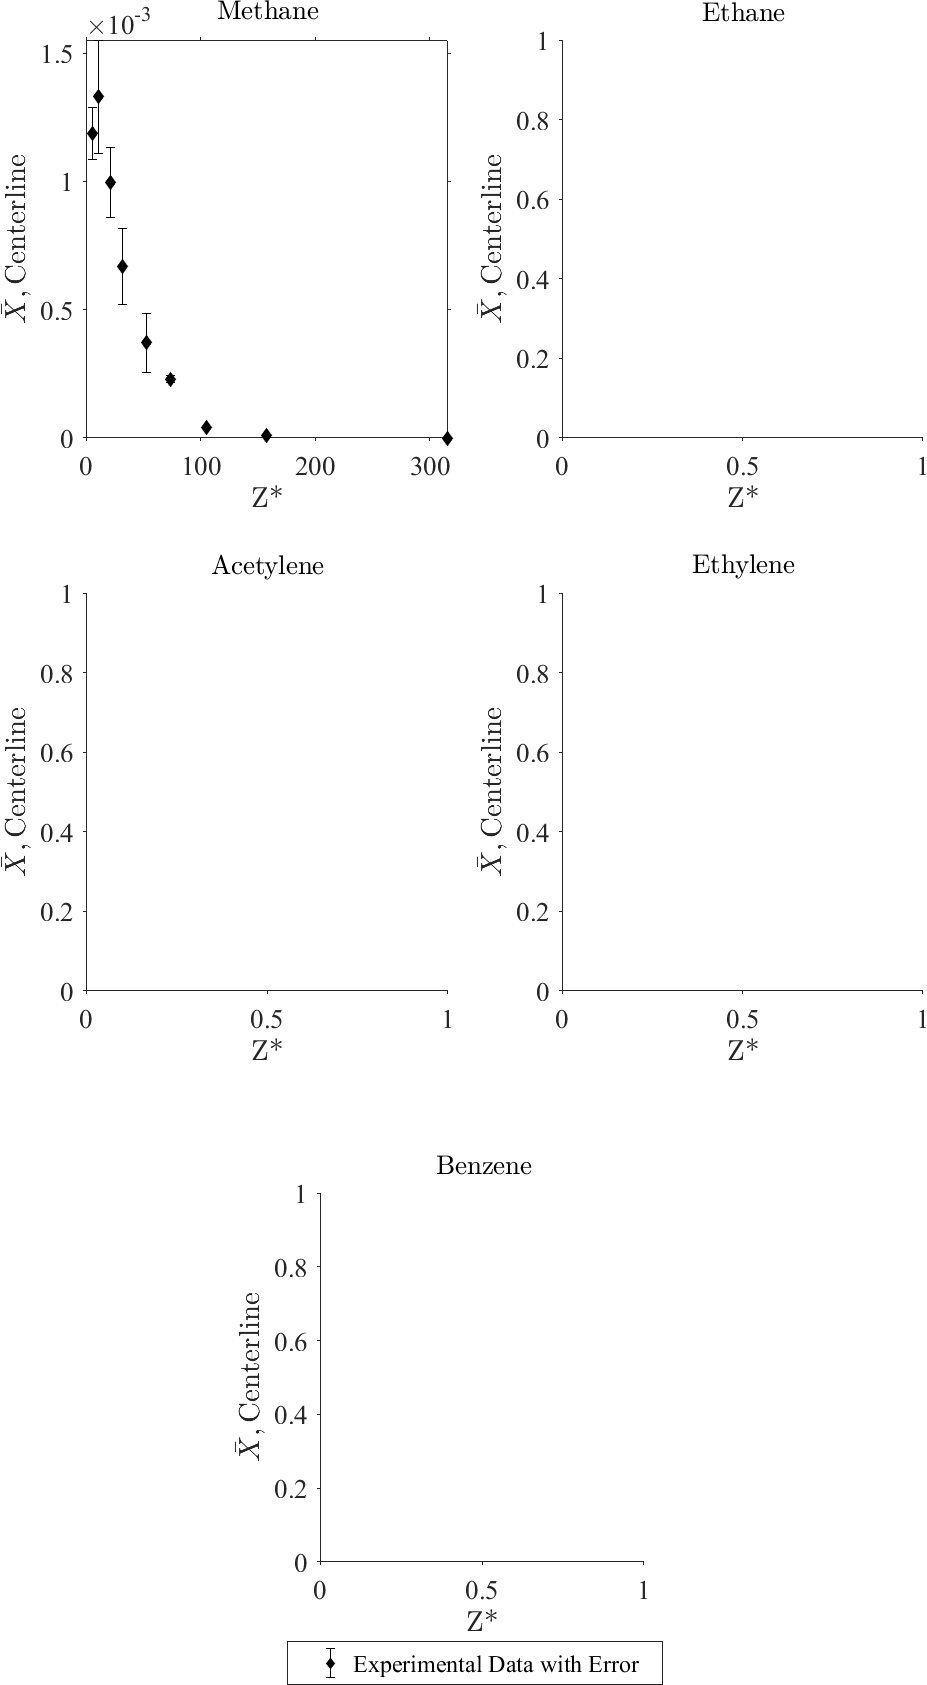
\includegraphics[width=10.0cm,keepaspectratio]{Methanol_Inter_MOL_FRAC_Plot.png}
	\caption[Plot of volume fractions, with error, of intermediate species identified in the methanol pool fire centerline as function of $Z^{*}$]{Plot of volume fractions of intermediate species identified in the methanol pool fire centerline as function of $Z^{*}$}
	\label{fig:Methanol_VOL_Frac_Inter}
\end{figure}
\pagebreak

\subsection{Ethanol}
\label{ssec:Ethanol_ALL_Vol_Frac}

\begin{figure}[!h]
	\centering
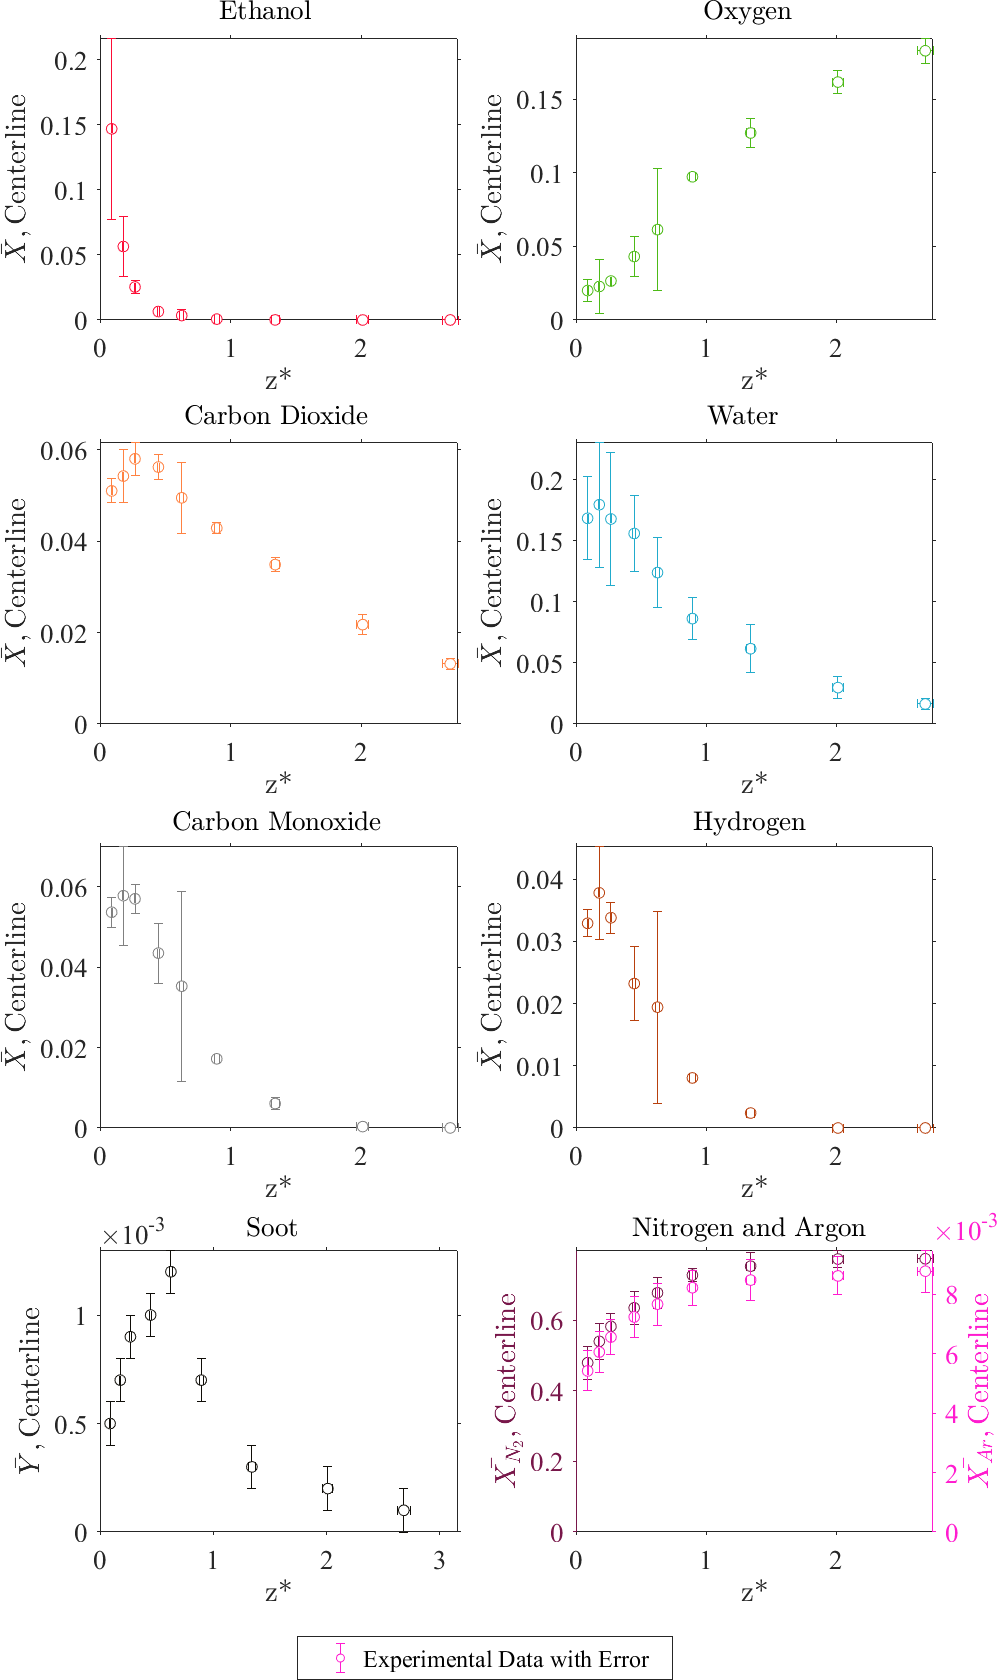
\includegraphics[width=10.5cm,keepaspectratio]{Ethanol_MOL_FRAC_Plot.png}
	\caption[Plot of volume fractions, with error, of major species identified in the ethanol pool fire centerline as function of $Z^{*}$]{Plot of volume fractions of major species identified in the ethanol pool fire centerline as function of $Z^{*}$}
	\label{fig:Methanol_VOL_Frac_Major}
\end{figure}
\pagebreak

\begin{figure}[!h]
	\centering
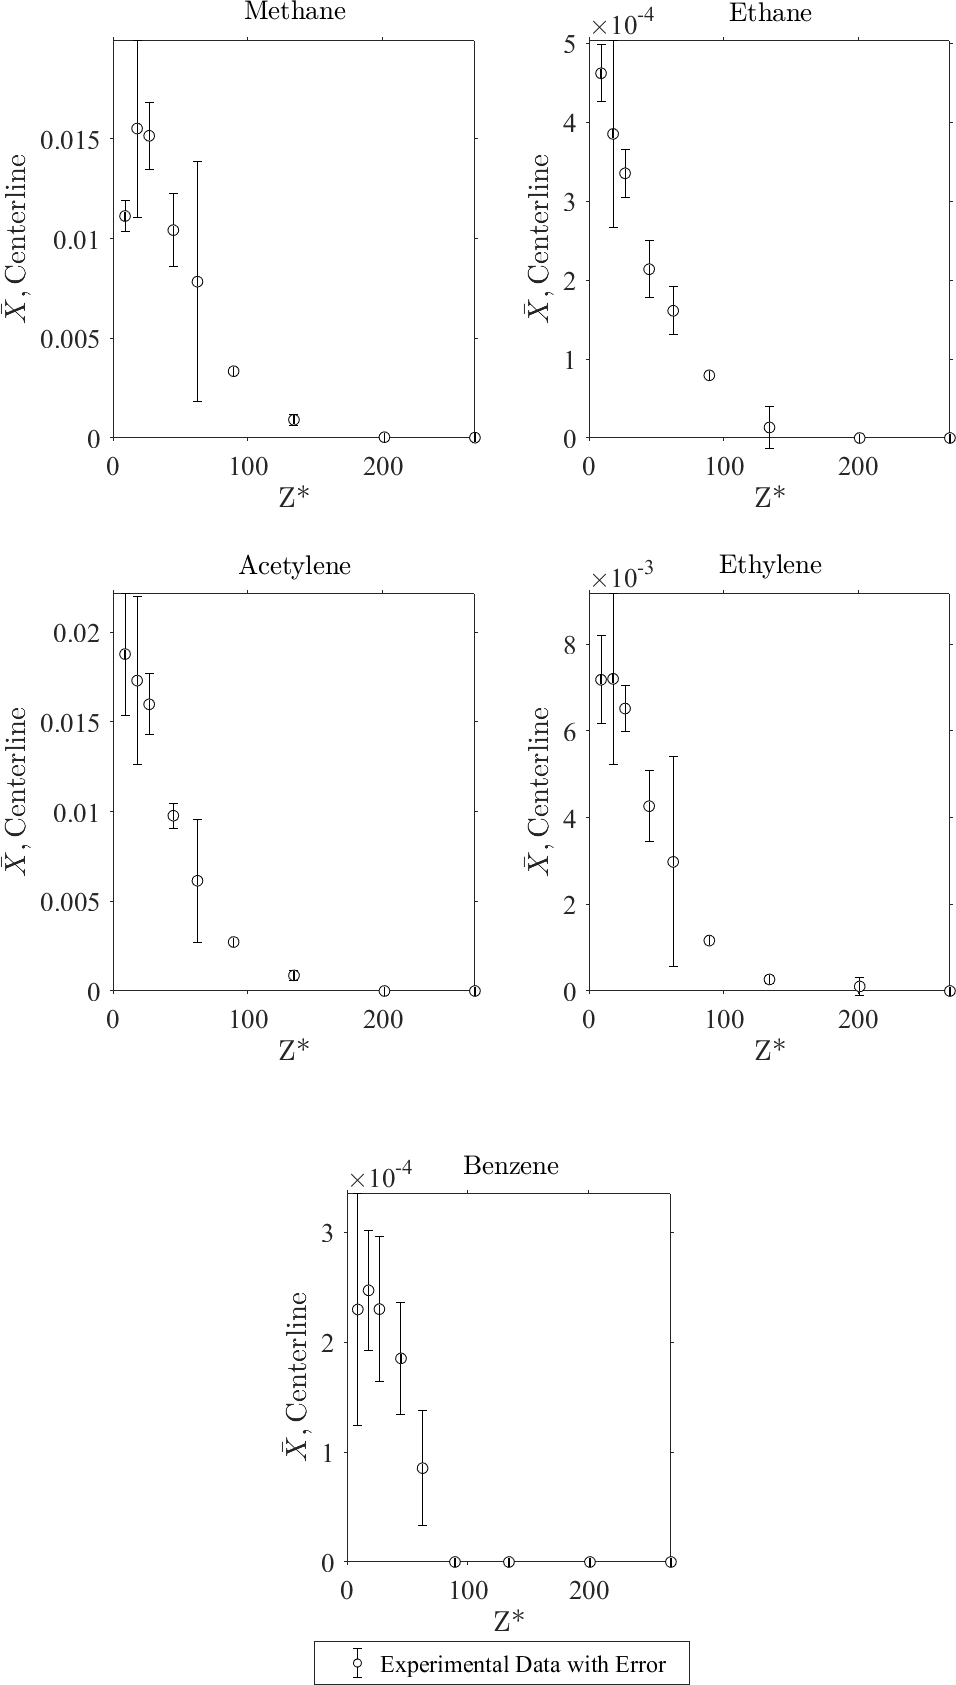
\includegraphics[width=10.5cm,keepaspectratio]{Ethanol_Inter_MOL_FRAC_Plot.png}
	\caption[Plot of volume fractions, with error, of intermediate species identified in the ethanol pool fire centerline as function of $Z^{*}$]{Plot of volume fractions of intermediate species identified in the ethanol pool fire centerline as function of $Z^{*}$}
	\label{fig:Methanol_VOL_Frac_Inter}
\end{figure}


\pagebreak
\subsection{Acetone}
\label{ssec:Acetonel_ALL_Vol_Frac}

\begin{figure}[!h]
	\centering
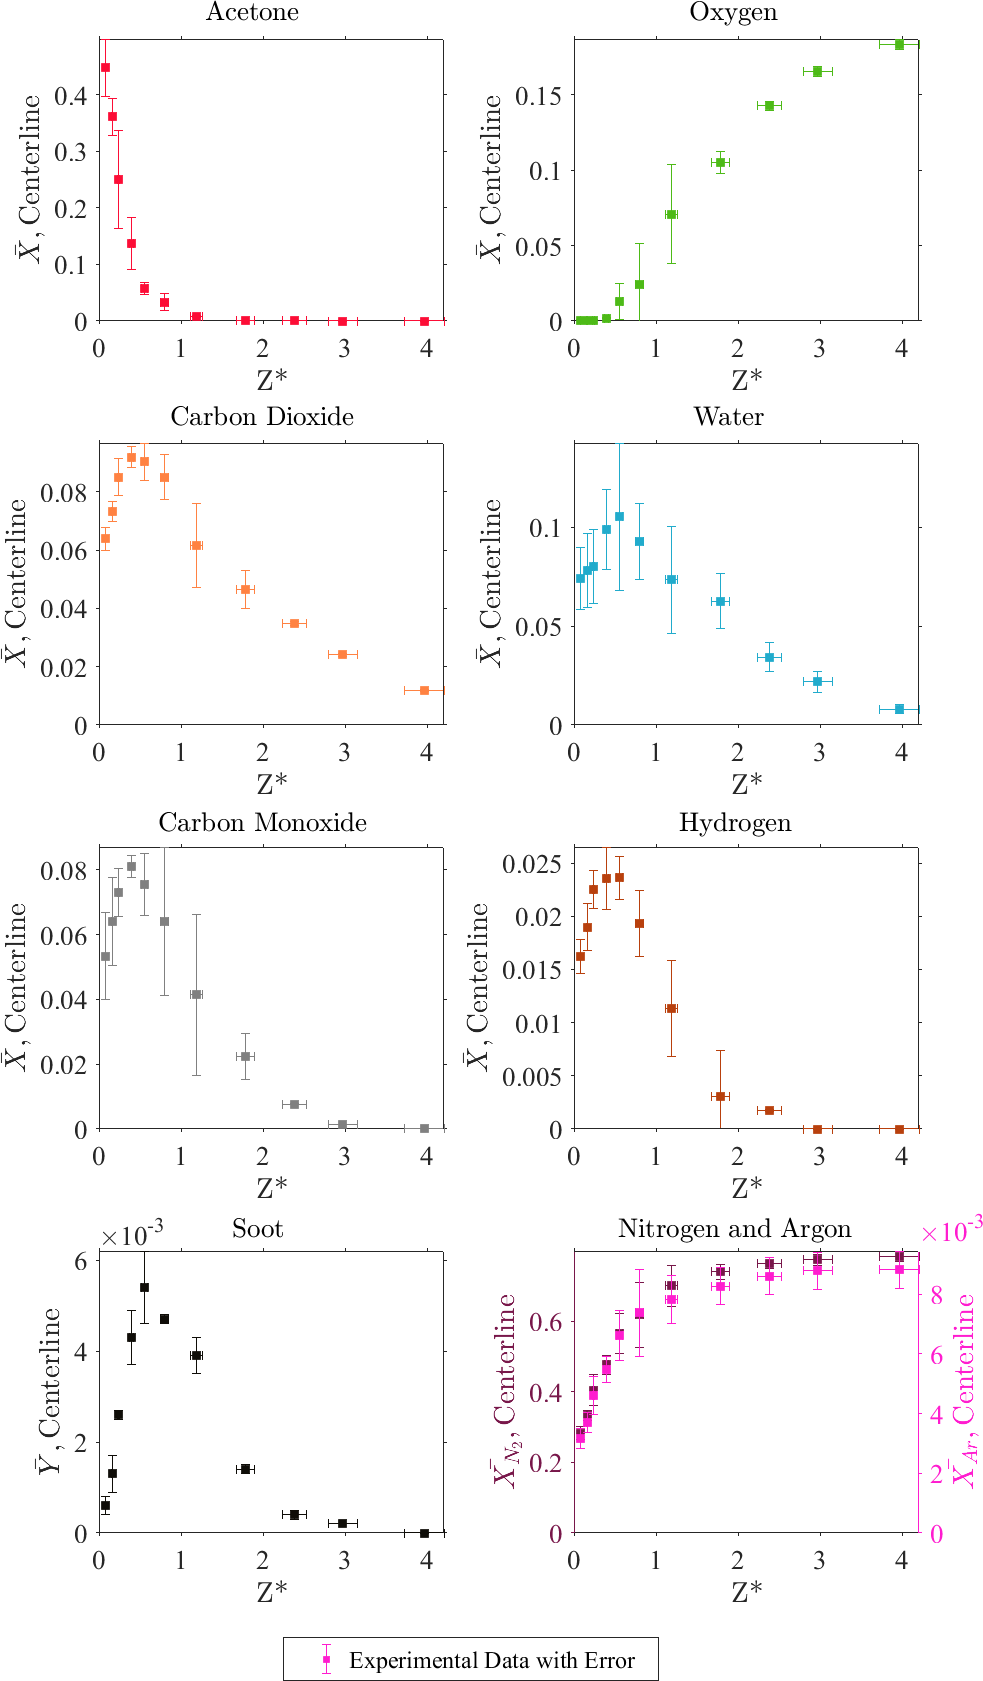
\includegraphics[width=10.0cm,keepaspectratio]{Acetone_MOL_FRAC_Plot.png}
	\caption[Plot of volume fractions, with error, of major species identified in the acetone pool fire centerline as function of $Z^{*}$]{Plot of volume fractions of major species identified in the acetonel pool fire centerline as function of $Z^{*}$}
	\label{fig:Methanol_VOL_Frac_Major}
\end{figure}

\begin{figure}[!h]
	\centering
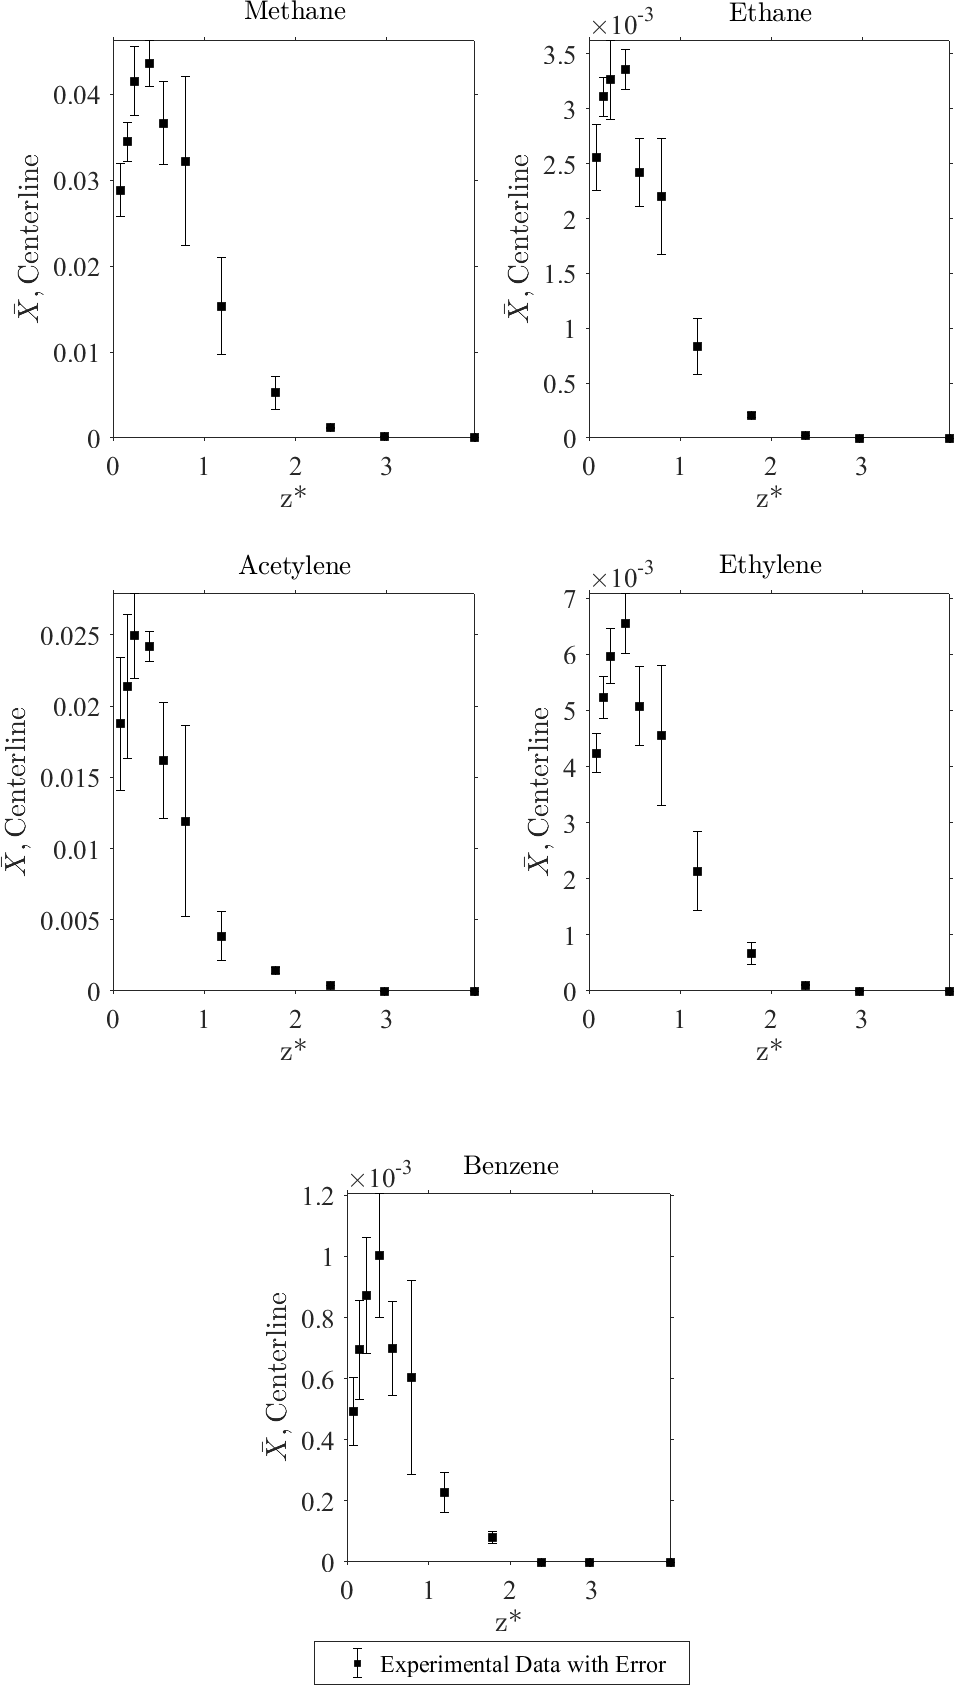
\includegraphics[width=10.0cm,keepaspectratio]{Acetone_Inter_MOL_FRAC_Plot.png}
	\caption[Plot of volume fractions, with error, of intermediate species identified in the acetone pool fire centerline as function of $Z^{*}$]{Plot of volume fractions of intermediate species identified in the acetone pool fire centerline as function of $Z^{*}$}
	\label{fig:Methanol_VOL_Frac_Inter}
\end{figure}

\pagebreak

\section{Figures of Averaged Mass Fractions of Centerline Measurements as a Function of Mixture Fractions for Methanol, Ethanol, and Acetone Fires}\label{sec:Mix_Frac_Figs}
\addcontentsline{toc}{section}{Appendix I: Figures of Averaged Mass Fractions of Centerline Measurements as a Function of Mixture Fractions for Methanol, Ethanol, and Acetone Fires}

\subsection{Methanol}
\label{ssec:Methanol_ALL_Mix_Frac}

\begin{figure}[!h]
	\centering
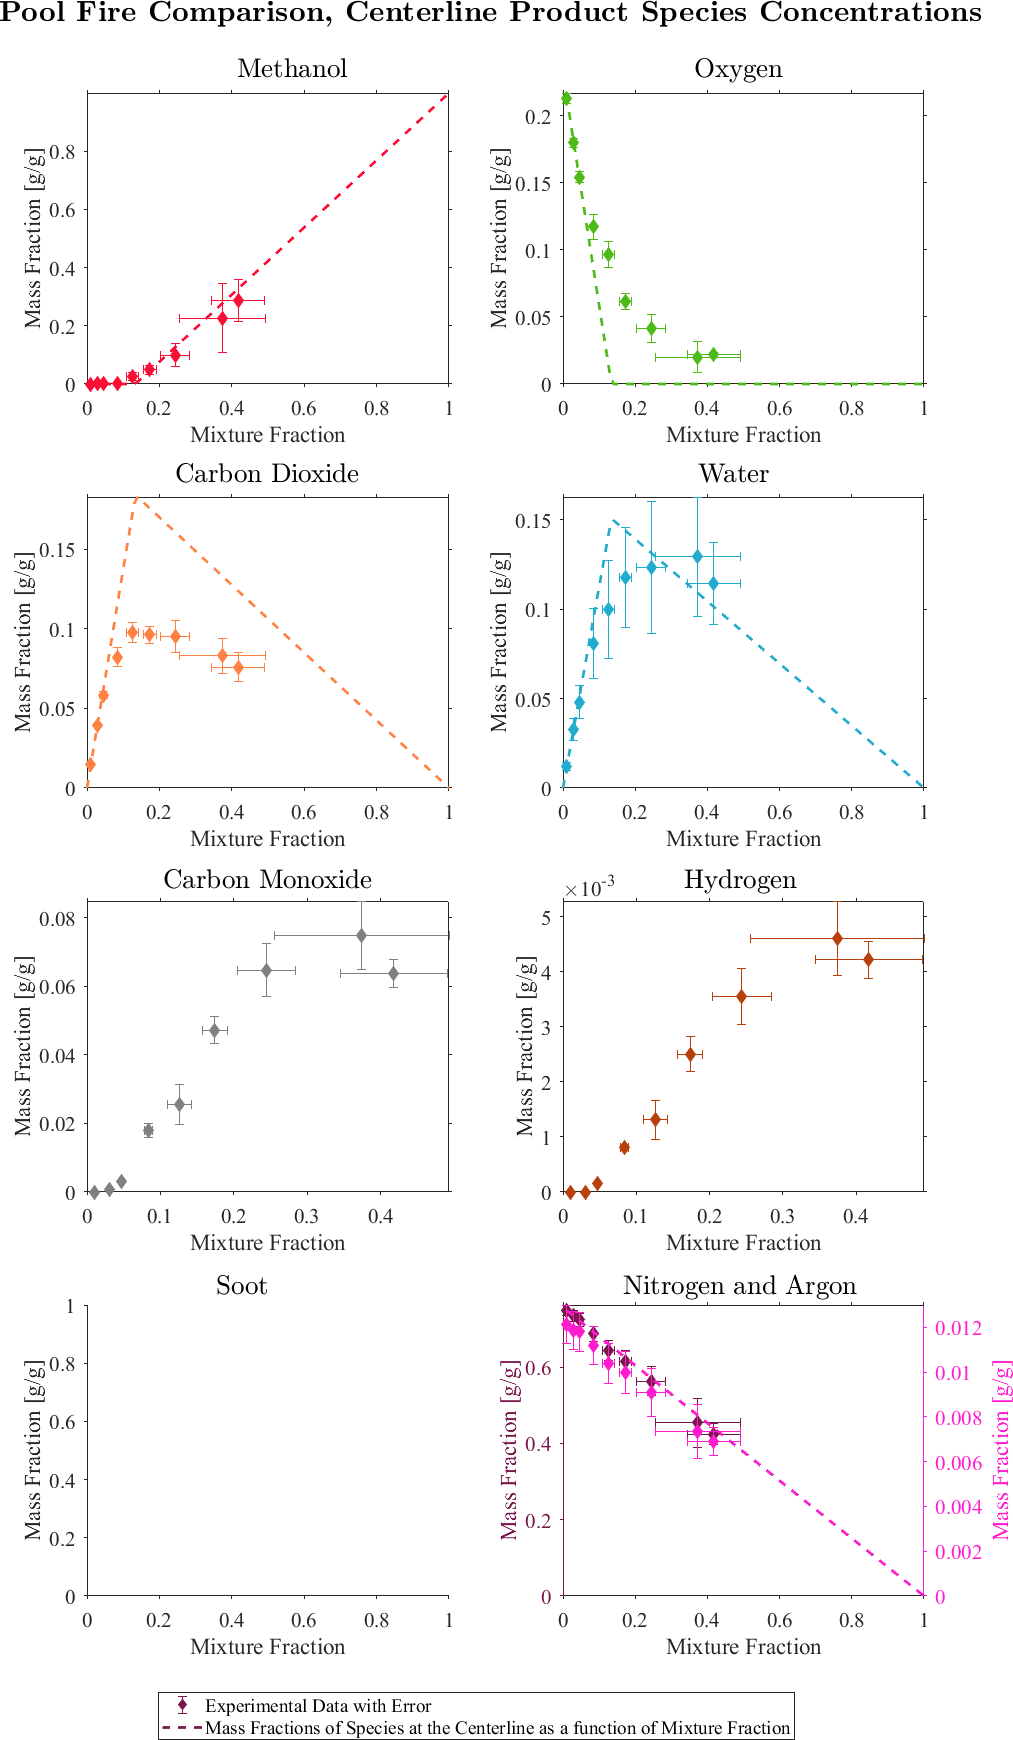
\includegraphics[width=10.0cm,keepaspectratio]{Methanol_Mixture_Fraction_Major_Plot.png}
	\caption[Plot of mass fractions, with error, of major species identified in the methanol pool fire centerline as function of mixture fraction]{Plot of mass fractions, with error, of major species identified in the methanol pool fire centerline as function of mixture fraction}
	\label{fig:Methanol_MIX_Frac_Major}
\end{figure}

\pagebreak

\subsection{Ethanol}
\label{ssec:Ethanol_ALL_Mix_Frac}
\begin{figure}[h!]
	\centering
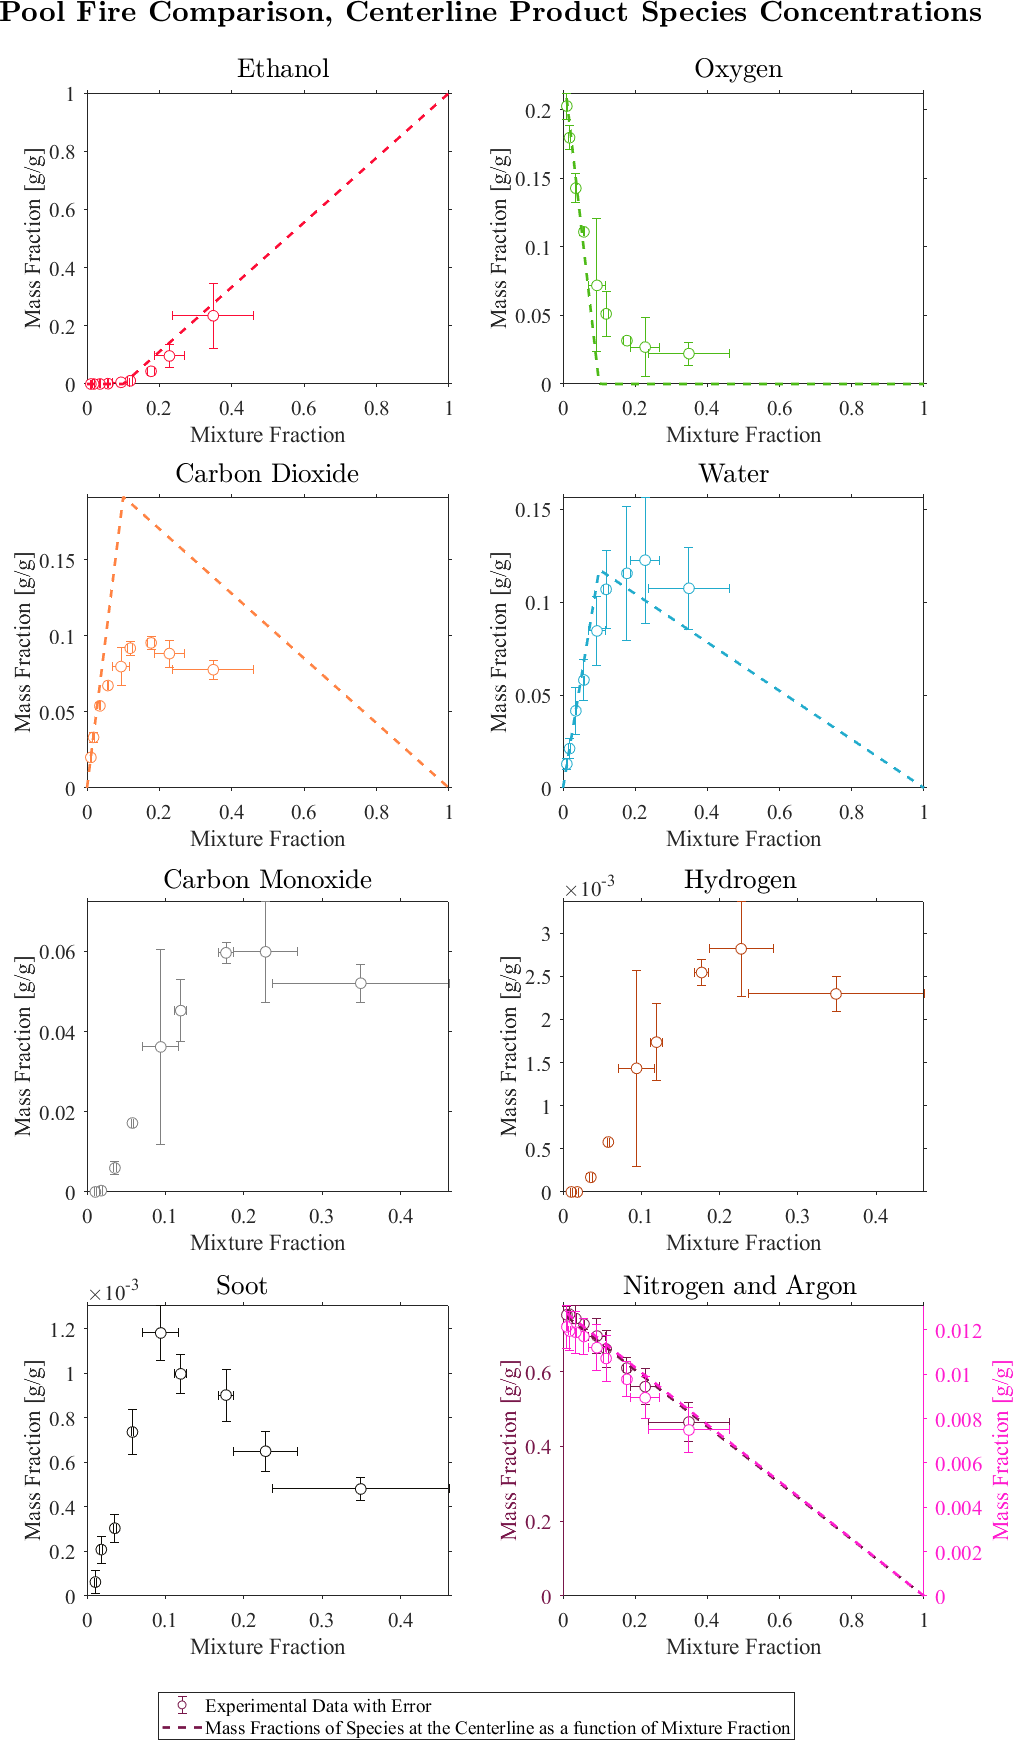
\includegraphics[width=10.0cm,keepaspectratio]{Ethanol_Mixture_Fraction_Major_Plot.png}
	\caption[Plot of mass fractions, with error, of major species identified in the ethanol pool fire centerline as function of mixture fraction]{Plot of mass fractions, with error, of major species identified in the ethanol pool fire centerline as function of mixture fraction}
	\label{fig:Ethanol_MIX_Frac_Major}
\end{figure}

\pagebreak

\subsection{Acetone}
\label{ssec:Acetone_ALL_Mix_Frac}
\begin{figure}[!h]
	\centering
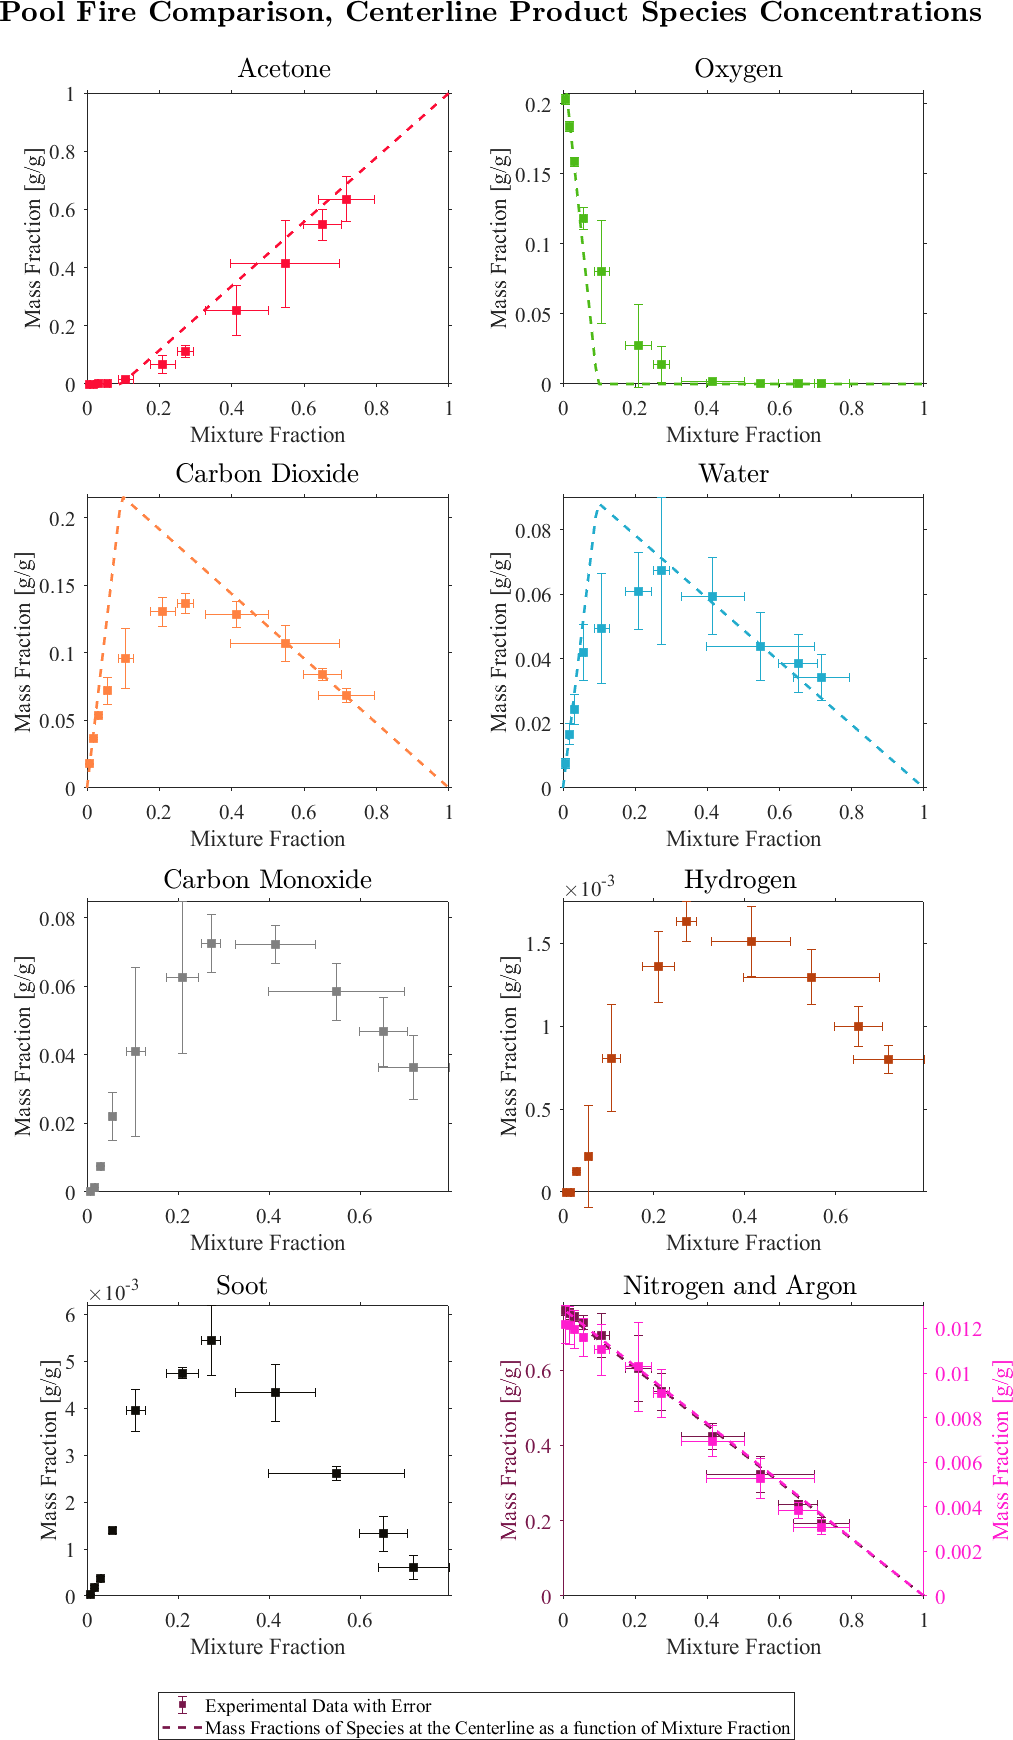
\includegraphics[width=10.0cm,keepaspectratio]{Acetone_Mixture_Fraction_Major_Plot.png}
	\caption[Plot of mass fractions, with error, of major species identified in the acetone pool fire centerline as function of mixture fraction]{Plot of mass fractions, with error, of major species identified in the acetone pool fire centerline as function of mixture fraction}
	\label{fig:Acetone_MIX_Frac_Major}
\end{figure}

\pagebreak

\section{Uncertainty Analysis of the Verification Scheme}\label{sec:Uncertainty_Ver_Scheme}
\addcontentsline{toc}{section}{Appendix J: Uncertainty of the Verification Scheme}
\subsection{Ratio of moles identified to moles injected }
\label{ssec:mole ratio}
The uncertainty of the ratio of the total number of moles identified by the TCD and MSD, $n_{\rm tot}$, to the number of moles injected into the GC/MSD, $n_{\rm inj}$, was calculated using the law of propagation of uncertainty and shown in the equation below:
\begin{equation}
\label{eq:mol_ratio_uncertainty}
u_{\scriptscriptstyle n_{\rm tot}/n_{\rm inj}} = \sqrt{\left(\frac{u_{\scriptscriptstyle n_{\rm tot}}}{n_{\rm inj}}\right)^2 + \left(\frac{-n_{\rm tot}~u_{\scriptscriptstyle n_{\rm inj}}}{{n_{\rm inj}^2}}\right)^2}
\end{equation}
The uncertainty of the total number of moles identified, $n_{\rm tot}$, is described in Section~\ref{ssec:Total Number of Moles Identified}. The uncertainty of the number of moles injected into the GC/MSD, $n_{\rm inj}$, is described in Section~\ref{ssec:Total Moles Injected into the GC/MSD for Calibation}.

\subsection{Carbon to Hydrogen Ratio}
\label{ssec:C2H_ratio}
The carbon to hydrogen ratio was calculated using Eqn.~\ref{eq:c2h_ratio} using the mass fraction of any quantified gas species that contained either carbon, $\bar{Y}_{i,C}$, or hydrogen, $\bar{Y}_{i,H}$.
\begin{equation}
\label{eq:c2h_uncertainty}
u_{\scriptscriptstyle {\rm C}/{\rm H}} = \sqrt{{\sum\left(\frac{\partial ({\rm C}/{\rm H})}{\partial \bar{Y}_{i,C}}\,u_{\scriptscriptstyle \bar{Y}_{i,C}}~{\frac{\textrm{W}_{C}}{\textrm{W}_{i,C}}} \right)}^2+{\sum\left(\frac{\partial ({C}/{H})}{\partial Y_{i,H}}\,u_{\scriptscriptstyle \bar{Y}_{i,H}}{\frac{\textrm{W}_{H}}{\textrm{W}_{i,H}}} \right)}^2}
\end{equation}
The uncertainty of the mass fractions of carbon and hydrogen containing species is described in Appendix~\ref{ssec:Uncertainty of Mass Fractions}.

\subsection{Stoichiometric Combustion Ratio}
\label{ssec:Pro_ratio}
The stoichiometric combustion ratio, $\text{SCR}$, was calculated from a ratio of volume fractions of combustion products, $\bar{X}_{i}$, identified by the TCD and TIC chromatograms. The uncertainty of $\text{SCR}$ was determined from the law of propagation of uncertainty:
\begin{equation}
\label{eq:c2h_ratio_uncertainty}
u_{\scriptscriptstyle \text{SCR}} = \sqrt{{\sum\left(\frac{\partial \text{SCR}}{\partial \bar{X}_{i}}\,u_{\scriptscriptstyle \bar{X}_{i}}\right)}^2}
\end{equation}
The uncertainty of the volume fractions is described in Appendix~\ref{sec:UncertaintyMoleFrac}.

\subsection{Inert Ratio}
\label{ssec:Inert_ratio}
The inert ratio was calculated from the ratio the Nitrogen and Argon volume fractions, $\bar{X}_{N_2}$ and $\bar{X}_{Ar}$, identified by the TCD and TIC chromatograms. The uncertainty of inert ratio was determined from the law of propagation of uncertainty:
\begin{equation}
\label{eq:inert_ratio_uncertainty}
u_{\scriptscriptstyle \bar{X}_{N_2}/\bar{X}_{Ar}} = \sqrt{{\left(\frac{u_{\scriptscriptstyle \bar{X}_{N_2}}}{\bar{X}_{Ar}}\right)}^2+{\left(\frac{-\bar{X}_{N_2}u_{\scriptscriptstyle \bar{X}_{Ar}}}{\bar{X}_{Ar}}\right)}^2}
\end{equation}
The uncertainty of the volume fractions is described in Appendix~\ref{sec:UncertaintyMoleFrac}.

\pagebreak
\end{document}
